\documentclass[journal]{IEEEtran}
\pdfoutput=1

\usepackage[T1]{fontenc}
\usepackage{cite}
\usepackage{amsmath,amssymb,amsfonts}
\usepackage{graphicx}
\usepackage{booktabs}
\usepackage{array}
\usepackage{etoolbox}
\makeatletter\patchcmd{\appendices}{\def\thesectiondis{APPENDIX \Alph{section}}.}{\def\thesectiondis{APPENDIX \Alph{section}}}{}{}\makeatother % the class sets a stray full stop here
\usepackage{textcomp}
\usepackage[hidelinks]{hyperref}
\usepackage{url}
\newcommand{\lmin}{\lambda_{\min}}
\newcommand{\lmax}{\lambda_{\max}}
\begin{document}
\title{Detection-Limited Eigenvalue Learning for Hybrid Quantum Linear System Solvers}
\author{Hikaru~Wakaura and Taiki~Tanimae%
\thanks{The authors are with QIRI (Quantum Integrated Research Institute Inc.), Tokyo 107-0061, Japan (e-mail: h.wakaura@qiri.co.jp; t.tanimae@qiri.co.jp).}%
\thanks{Corresponding author: Hikaru Wakaura (e-mail: h.wakaura@qiri.co.jp).}}

\maketitle

\begin{abstract}
Hybrid quantum linear system solvers of the Harrow--Hassidim--Lloyd (HHL) type learn the eigenvalues that carry weight in the input and then run a short clock register. In the regimes tested, the detection of weak spectral components decides the choice of the learning estimator. In a counting model built on known scalings, a component of weight $w$ needs about $(w+w_{\rm fl})/w^2$ samples, with $w_{\rm fl}$ the weight leaking into its label: $1/w^2$ for single-ancilla mixture estimators and $1/w$, down to a leakage floor of a few per cent, when a clock register labels each shot (Projective HHL). Recycled sequential HHL measures one copy of the input repeatedly with one ancilla and labels it by its own Bayesian posterior; its label error is tuned by a stopping threshold, not bounded. On four systems with calibrated ancilla noise it gives a lower median solution infidelity than Projective HHL within the same evolution time in all eight settings, by factors from $2$ to $3\times10^3$; neither is uniformly better for the compliance. Without dephasing it alone resolves, in most runs, the weak component at the smallest eigenvalue of a 9-bus power-flow problem; at ten times that budget it reproduces the ridge readout of a reservoir computer on three series in all runs, at a resolution compared afterwards. With dephasing the coherent clock limits every solver tested. A depolarised system register corrupts the learned weights: in a jump model the compliance error is $5.6\%$ at a lifetime more than twenty times the longest copy.
\end{abstract}

\begin{IEEEkeywords}
Bayesian phase estimation, eigenvalue estimation, hybrid quantum--classical algorithms, power flow, quantum linear system algorithms, quantum phase estimation
\end{IEEEkeywords}

\section{Introduction}
\label{sec:introduction}
\IEEEPARstart{S}{olving} linear systems $A\vec x=\vec b$ underlies most of scientific computing, and the HHL algorithm \cite{HHL2009} and its successors \cite{Gilyen2019,Martyn2021,Morales2026} promise to prepare the normalised solution state $|x\rangle$ with a cost that is polylogarithmic in the dimension. The promise comes with well-known conditions on sparsity, condition number $\kappa$, state preparation and read-out \cite{Morales2026,Pareek2026}, and with a practical obstacle that dominates every attempt to run the algorithm on present hardware: the eigenvalue estimation stage. In the textbook circuit the eigenvalues are written coherently into a clock register by QPE, and the depth of that register grows exponentially with the number of precision bits, which empirical studies identify as the most severe bottleneck on noisy devices \cite{Marfany2024}.

Hybrid HHL schemes \cite{Lee2019,Yalovetzky2024,Morgan2025,Gao2021} side-step the problem by learning the eigenvalues $\{\lambda_j\}$ that carry weight in the input, $|b\rangle=\sum_j\beta_j|u_j\rangle$, in a separate classical post-processed experiment, and then running a short clock whose rotation angles are set from the learned values. The learning experiment has been a sampled QFT-type QPE \cite{Lee2019,Yalovetzky2024,Morgan2025}, run in \cite{Yalovetzky2024} in its semiclassical form with one ancilla, or, for eigenvalues that are exact binary fractions, an iterative phase estimation \cite{Gao2021}. In parallel, the early fault-tolerant literature has produced single-ancilla eigenvalue estimators that reach the Heisenberg limit without eigenstate preparation, including multi-order time-series methods \cite{Dutkiewicz2022,OBrien2019}, QCELS \cite{QCELS2023,DingLin2023}, robust multiple-phase estimation \cite{RMPE2023}, Gaussian-filtered search \cite{QMEGS2024}, and measurement-backaction schemes \cite{Jin2023}. To our knowledge these continuous-valued estimators have not been compared as learning stages of a linear solver for an input with an unknown number of weighted components, which is the question addressed here. Methods that avoid phase estimation altogether, a variational solver \cite{BravoPrieto2023} and, for a forecasting task, quantum reservoir computing \cite{Fujii2017}, quantum circuit learning \cite{Mitarai2018} and decoded quantum interferometry \cite{Jordan2025}, are included as further baselines (Sec.~\ref{sec:vqls}). Table~\ref{tab:position} lists the eight learning stages of the application tests (three mixture estimators, QPE histograms of three register sizes and the two labelled schemes) with what each requires.

This paper makes three points. The first is a detection criterion for the learning stage, built on scalings that are known for single estimators (Sec.~\ref{sec:setting}). For a non-eigenstate input a single-ancilla Hadamard test measures the mixture $\sum_jw_j\cos(\lambda_jt+\theta)$; the derivative of the outcome probability with respect to a weight $w_j$ does not depend on $w_j$, so for a contrast below one the Fisher information per shot on each weight is $O(1)$, the relative weight error is $\sim1/(w_j\sqrt S)$, and a component can be told from its absence only when $S\gtrsim w_j^{-2}$. A scheme that labels each shot by a short coarse QPE instead counts the component with Poisson statistics, relative error $\sim1/\sqrt{w_jS}$ and $S\gtrsim w_j^{-1}$, down to a floor set by clock leakage. The eigenvalue precision of a detected component is a secondary quantity: its local information scales as $w_j^2$ for the mixture and as $w_j$ with labelling, and at the budgets studied it is the binding constraint only for the smallest eigenvalues under dephasing (Sec.~\ref{sec:solver}). Because a missed component at a small eigenvalue carries a large share of the solution, detection decides the solution fidelity. We first benchmark such a register-labelled learning stage, which keeps the single-ancilla refinement but labels each shot by a coarse QPE, against mixture estimators and sampled QPE under dephasing.

The second point is that the floor belongs to the clock register and not to labelling. If one copy of $|b\rangle$ is kept and measured repeatedly with a single ancilla, every measurement operator is a function of $A$, and the probability of a record is a weighted product over the measurements, as if one eigencomponent had been drawn with probability $w_j$ \cite{OBrien2019}. This back-action is the basis of the channel framework of \cite{Jin2023}, whose adaptive scheme reads binary digits, and of solvers built on iterative phase estimation for eigenvalues that are exact binary fractions \cite{Gao2021}.

We combine it with known Bayesian tools into a learning stage in which each copy is labelled by its own posterior and stopped at a posterior-tail threshold, so that the label has no $1/d^2$ tail, the resolution is set by evolution time rather than by a register size, and the number of components need not be known. The measurement settings maximise the rate of expected variance reduction \cite{deNeeve2025,McMichael2021}, evaluated in closed form from Fourier moments of the posterior, and evolution time can be allocated only to components that are above their precision target. The stopping threshold is not a proven error bound; we measure the label error, including under a mismatched noise model, and we test by an ablation whether the advantage survives a change of the time allocation.

We name the two labelled schemes by the hybrid solver they define. \emph{Projective HHL} learns with the projective estimator, in which the clock outcome of a short QPE labels the shot and collapses the input approximately onto the labelled eigencomponent; this is the register-labelled learning of the hybrid schemes cited above with a refinement measurement added. \emph{Recycled sequential HHL} learns with the sequential estimator, in which one copy of the input is recycled through sequential single-ancilla phase estimation and labelled by its own posterior. In column headings ``projective'' and ``sequential'' stand for the two. The names denote the configurations compared here and not new complete solvers: unless a real clock register is stated, the solution fidelity quoted for either is that of an idealised solver that applies the inverse of the learned eigenvalue nearest to each eigencomponent exactly.

The third point is that for a sparse spectral measure the learning stage already answers most questions asked of the solver. That $\langle b|f(A)|b\rangle=\int f\,d\mu_b$ is the spectral theorem, and estimating such integrals from an approximate cumulative distribution function is the route of Lin and Tong \cite{LinTong2022}, and a binned estimate of the measure from a single-ancilla time series is that of \cite{Somma2019}; what we add is the atomic case, in which the measure has few atoms and is represented by learned eigenvalues and weights, so that the compliance $\vec b^{\mathsf T}A^{-1}\vec b$, the energy of the solution and its mode weights follow with the per-atom weight error $\sqrt{w_j/S}$ rather than with a uniform error on the distribution function, and a polarisation identity with three further input states extends the construction to linear functionals $\langle v|A^{-1}|b\rangle$. No polynomial transformation and no post-selection are needed, and with the sequential estimator no clock register either. We compare this with two model-free estimators built from the same Hadamard tests, a thresholded time-evolution Krylov solver \cite{YuZhou2026,Park2026} and the randomised Fourier representation of $A^{-1}$, and find the regime of few weighted components in which the atomic representation wins. Only observables that are not diagonal in the eigenbasis still need the quantum back end; there we return the learned spectrum to a real clock, uniform or tapered \cite{HHL2009,Rendon2022,Patel2026,Kristjuhan2026}, and to spectrally corrected QSVT inversion \cite{Suresh2026}, and quantify what it buys and what it cannot repair.

Finally we apply all estimators to the DC power-flow problem of standard 9-, 14- and 30-bus test systems \cite{Zimmerman2011}, a linear system on which HHL-type solvers have been run for three to nine buses \cite{Eskandarpour2020,Eskandarpour2021,GaoPF2022}, to see which conclusions survive on spectra that were not chosen for the purpose (Sec.~\ref{sec:grid}). A second test is the readout training of a small reservoir computer for three nonlinear time series, a ridge-regression system \cite{Wiebe2012,Jaeger2004} in which components that hold less than $10^{-3}$ of the weight carry up to $72\%$ of the solution (Sec.~\ref{sec:series}). The result is a design rule for the learning stage and not a claim of advantage: every test system is solved classically at negligible cost, the noise model contains ancilla noise only, and an end-to-end analysis finds no practical advantage of quantum linear solvers for DC power flow \cite{Pareek2026}.

The paper is organised as follows. Section~\ref{sec:setting} states the setting and the detection law. Section~\ref{sec:stages} defines the three learning stages and Sec.~\ref{sec:bench} benchmarks them. Section~\ref{sec:solver} uses the learned measure as a solver for observables, and Sec.~\ref{sec:return} returns the spectrum to a solver with a real clock register. Section~\ref{sec:grid} applies all estimators to DC power-flow problems and Sec.~\ref{sec:series} to the readout training of a reservoir computer, Sec.~\ref{sec:vqls} adds baselines that do not use phase estimation, Sec.~\ref{sec:system} gives the system register a finite lifetime, and Sec.~\ref{sec:disc} gives the conclusions and the limitations.

\section{Setting and the detection law}
\label{sec:setting}

Let $A$ be Hermitian with eigenpairs $(\lambda_j,|u_j\rangle)$, $0<\lmin\le\lambda_j\le\lmax\le1$, $\kappa=\lmax/\lmin$, and let $w_j=|\beta_j|^2$ with $\sum_jw_j=1$ be the weights of the $m$ distinct eigenvalues on the support of $|b\rangle$. The single-ancilla circuit (ancilla $|+\rangle$, controlled $e^{-iAt}$, phase $\theta$, Hadamard, measurement) returns outcome 0 with probability
\begin{equation}
p(t,\theta)=\tfrac12+\tfrac12\,c(t)\sum_jw_j\cos(\lambda_jt+\theta),
\label{eq:p}
\end{equation}
where $c(t)=(1-p_d)e^{-t/T_2}$ is the contrast under depolarising rate $p_d$ and control-qubit dephasing time $T_2$; we take $c$ to be calibrated.

\emph{Assumptions.} Four assumptions are used throughout. (i)~$A$ is Hermitian and scaled so that its spectrum lies in $(0,1]$. (ii)~The controlled evolution $e^{-iAt}$ is exact for every $t$, and cost is counted as total evolution time. (iii)~Noise acts on the ancilla only, through the contrast $c(t)$, which is known. (iv)~The smallest gap $\Delta_{\min}$ of the spectrum is known; it fixes the register of Projective HHL and the resolution of Recycled sequential HHL. The weights $w_j$ are unknown, no lower bound on a weight is assumed, and the number of weighted components is not supplied to the two labelled estimators (the projective one takes the dimension as an upper limit). Sections~\ref{sec:bench} and \ref{sec:system} test departures from (iii), a mismatched contrast and a system register with a finite lifetime, and Sec.~\ref{sec:disc} lists what (ii) and (iii) leave out.

Five statements follow (proofs in Appendix~\ref{app:proofs}).

\emph{Detection and weight law (mixture).} On the simplex a change of $w_j$ is absorbed by the other weights, so $\partial p/\partial w_j=\tfrac12c(\cos\varphi_j-\bar g)$ with $\varphi_j=\lambda_jt+\theta$ and $\bar g$ the cosine of the absorbing components; this does not depend on $w_j$ and is at most $c$ in magnitude, so the Fisher information of one shot on the weight $w_j$ is at most $c^2/[p(1-p)]\le4c^2/(1-c^2)$, an $O(1)$ number when $c<1$. For any unbiased estimator of a resolved component, $\sigma(\hat w_j)\ge1/(2c\sqrt{\kappa_pS})$ with $\kappa_p=\overline{[4p(1-p)]^{-1}}\le(1-c^2)^{-1}$, so the relative weight error is $\sim1/(w_j\sqrt S)$ and a component is distinguishable from absence only when $w_j\sqrt S$ exceeds a threshold $z$ that increases with the number of frequency bins searched: $S\gtrsim z^2/w_j^2$. The dependence on the weight has precedents for single estimators: a time-series estimator was found numerically to have an error proportional to $1/(A_0\sqrt N)$ for a target of weight $A_0$ and $N$ experiments \cite{OBrien2019}, and the number of samples in the guarantee of the Gaussian-filtered search grows as $(p_{\min}-p_{\rm tail})^{-2}$, with $p_{\min}$ the smallest dominant weight and $p_{\rm tail}$ the total weight of the rest \cite{QMEGS2024}. The statement here is a necessary condition in a local model, for any unbiased estimator on these statistics; it is not a finite-sample guarantee of detection.

\emph{Detection and weight law (labelled).} If each shot carries a label that identifies the eigencomponent, the number of shots with label $j$ is binomial with mean $w_jS$, so $\sigma(\hat w_j)=\sqrt{w_j(1-w_j)/S}$, the relative error is $\sim1/\sqrt{w_jS}$, and the probability of never seeing the component is $(1-w_j)^S$: $S\gtrsim\ln(1/\delta)/w_j$ suffices. The sampled coherent clock of hybrid HHL is such a labelled scheme, which is why it does not suffer from the mixture law. That resources of order $1/w_j$ are needed by any scheme was noted in \cite{OBrien2019}, and for random input states, whose weights are $1/M$ on average in dimension $M$, a register that separates the eigenvalues detects all of them with a number of shots of order $M\log M$ when its size is polynomial in $M$ \cite{Izumi2026}. The two laws differ by the factor $w_j$ in the information, and this is the whole content of the ``$w_j$ versus $w_j^2$'' statement: it concerns detection and relative weights, not absolute weights and not, at the budgets considered here, eigenvalues. Nor is it a statement about the Heisenberg limit, which is the scaling of the total evolution time with the precision of an eigenvalue that has been resolved; the two laws count the samples needed before a component of weight $w_j$ is resolved at all.

\emph{A counting model.} The two statements can be read in one counting model. Let a labelling procedure assign a sample of component $j$ to the label of $j$ with probability $\alpha_j$ (its acceptance) and let $w_{\rm fl}$ be the total probability that a sample of another component receives that label. The count in the label is binomial with success probability $p_j=\alpha_jw_j+w_{\rm fl}$. If the background is not known the component is visible only for $\alpha_jw_j\gtrsim w_{\rm fl}$, a floor that does not decrease with $S$; if $\alpha_j$ and $w_{\rm fl}$ are known and the background is subtracted, a signal of $z$ standard deviations needs
\begin{equation}
S\ge z^2\,\frac{p_j(1-p_j)}{\alpha_j^2w_j^2}\approx z^2\,\frac{w_j+w_{\rm fl}}{w_j^2},
\label{eq:count}
\end{equation}
the last form for $\alpha_j\approx1$ and rare labels. This is a signal-to-noise criterion, not a finite-sample test with stated error rates. For a uniform clock register $w_{\rm fl}=\sum_{k\ne j}w_k\sum_{y\in Y_j}|a_{ky}|^2$ with $a_{ky}$ the clock amplitudes and $Y_j$ the bins assigned to the label (the peak bin and its two neighbours in the tests below), a few per cent next to a strong component and dependent on the instance, and $\alpha_j$ is the probability of the bins assigned to the component (on the planted-component test below, $0.57$ and $0.79$ for the peak bin of a five-bit register and $0.88$ and $0.93$ for the three bins around it). For the sequential estimator of Sec.~\ref{sec:stages}, $w_{\rm fl}$ is set by the stopping threshold and is measured in Sec.~\ref{sec:bench}. Mixture statistics have no label; their weight law has the scaling of \eqref{eq:count} with $w_{\rm fl}=O(1)$, which is an analogy and not an identity of the two observation models. In this model the cost of a learning stage is decided by how small it makes $w_{\rm fl}$ and by what a sample costs.

\emph{Eigenvalue information (secondary).} The Fisher information matrix of one setting with respect to the eigenvalues is $I_{jk}=c^2t^2w_jw_k\sin\varphi_j\sin\varphi_k/[4p(1-p)]$, of rank one; averaged over $\theta$ and over a time window wider than the inverse gaps it is approximately diagonal with $\bar I_{jj}\asymp c^2\overline{t^2}w_j^2$ (bounds in Appendix~\ref{app:proofs}), so a detected component can be refined to $\sigma_j\asymp1/(w_jT\sqrt S)$ by the mixture and to $\sigma_j\asymp1/(\sqrt{w_j}T\sqrt S)$ with labels, the labelled single-cosine information per shot being $t^2(1-\sqrt{1-c^2})$ after averaging over the phase. With $T$ of a few hundred and $S=10^4$ these errors are below $10^{-3}$ for every $w_j\ge0.03$ and are not what limits the solver.

\emph{Error propagation.} For the solver output $|\hat x\rangle\propto\sum_j(\beta_j/\hat\lambda_j)|u_j\rangle$ with $\hat\lambda_j=\lambda_j+\delta_j$, write $q_j=(w_j/\lambda_j^2)/\sum_k(w_k/\lambda_k^2)$ for the share of component $j$ in $\|x\|^2$ and $e_j=\delta_j/\lambda_j$. Then
\begin{equation}
1-F=\sum_jq_je_j^2-\Big(\sum_jq_je_j\Big)^2+O(\|e\|^3),
\label{eq:prop}
\end{equation}
where the second term is the cancellation of errors parallel to the solution (a common relative error of all eigenvalues leaves the normalised state unchanged). To this order $1-F\le\sum_jq_je_j^2$, and for independent zero-mean errors $\mathbb E[1-F]=\sum_jq_j(1-q_j)\mathbb E[e_j^2]$. A component that is missed altogether, or frozen at a coarse value, contributes instead $q_j(1-q_j)(r-1)^2/[1+q_j(r^2-1)]$ with $r=\lambda_j/\lambda_{\rm nn}$, where $\lambda_{\rm nn}$ is the eigenvalue it is merged with and the other components are exact; this is $\approx q_j(r-1)^2$ to leading order in $q_j$, $O(q_j)$ rather than $O(e_j^2)$. On the Poisson $N=8$ system used below the component with $w=0.032$ at $\lambda=0.031$ has $q=0.89$: missing it costs most of the fidelity, while refining it beyond $10^{-2}$ changes little. A weak neighbour that is merged with it is amplified by the small eigenvalue: the $w=0.006$ component at $\lambda=0.121$ ($q=0.011$) rotated with $\lambda=0.031$ costs $0.076$. Detection, not precision, decides the fidelity, and the two laws above decide detection.

\emph{Tracking and unwrapping (heuristic).} For a multi-stage mixture estimator that doubles the evolution time between rounds of $S_r$ shots, staying in the correct phase basin requires $\sigma_jT_{r+1}\lesssim0.4$ and hence a growth factor $f\lesssim c_uw_j\sqrt{S_r}$; components with $w_j\lesssim f/(c_u\sqrt{S_r})$ cannot follow and are frozen (Appendix~\ref{app:proofs}). This is a property of that estimator class, not a lower bound, and robust multi-peak methods \cite{RMPE2023,QMEGS2024} are not bound by it.

\section{Three learning stages}
\label{sec:stages}

\emph{Mixture estimators.} We implement two representatives of the single-ancilla family: a multi-level least-squares estimator in the spirit of MM-QCELS \cite{DingLin2023}, which refits all eigenvalues and weights on time grids $t_n=n\tau_\ell$ with $\tau_\ell=\tau_02^\ell$, and a Gaussian-filtered search in the spirit of QMEGS \cite{QMEGS2024}, which samples $t\sim\mathcal N(0,T^2)$ and reads eigenvalues from the peaks of $\overline{\mathrm{Re}[Z_ne^{ixt_n}]}$. The application tests add a third, listed as ``Bayesian clock'': a matrix pencil on the time series $\sum_jw_je^{i\lambda_jt}$ \cite{OBrien2019} gives starting values, and rounds whose evolution time at most doubles refit all eigenvalues and weights, the multi-stage scheme of the tracking argument of Sec.~\ref{sec:setting}. All three see \eqref{eq:p}, inherit the mixture eigenvalue rate and are given the dimension as the number of components.

\emph{Projective HHL: the projective estimator.} Each shot runs an $n_c$-bit QPE with $t_0=2\pi/1.25$ whose clock outcome $y$ labels a component (probability $w_j$) and collapses the register; the same shot then applies the Hadamard test at an adaptive time $t=0.6/\sigma_{j}$ and phase $\theta=-\hat\lambda_jt-\pi/2$ to the collapsed state and updates a one-dimensional grid posterior for that component (the Wiebe--Granade rule \cite{WiebeGranade2016}, tempered to absorb mislabelling). The number of coarse bits is set by the resolution needed to separate the spectrum and by the coherence budget,
\begin{equation}
n_c=\min\big\{\lceil\log_2(2\lmax/\Delta_{\min})\rceil,\ \lfloor\log_2(T_2/t_0)\rfloor\big\},
\label{eq:nc}
\end{equation}
so that the coherent part is governed by the spectral resolution $\Delta_{\min}$ and not by the target precision $\varepsilon$; the precision is carried by the incoherent refinement, whose maximal time is capped at $T_2$ ($2T_2$ in Table~\ref{tab:learn}; $2000$ without dephasing, the window of the mixture baselines). Near-degenerate pairs below the coarse resolution are treated as one cluster. The construction is the explicit-register version of the backaction steering of \cite{Jin2023}. A finite clock does not project exactly: outcome $y$ leaves the register in $\propto\sum_j\beta_ja_{jy}|u_j\rangle$, so the refinement sees a mixture with purity $\pi_j=w_j|a_{jy}|^2/\sum_kw_k|a_{ky}|^2$ in the bin of component $j$, the effective weight in the labelled law is $w_j\pi_j^2$, and a weak component whose bin receives the $1/(\pi^2d^2)$ tail of a strong one $d$ bins away is lost below a floor $w_j\lesssim\sum_{k\ne j}w_k\sum_{y\in Y_j}|a_{ky}|^2$ that does not decrease with $S$. This leakage floor, not the shot count, is what limits the labelled scheme, and it is the mechanism behind the two-group results reported below.

\emph{Recycled sequential HHL: the sequential estimator.} The leakage floor is a property of the finite register, and it is avoided by not using one. A copy of $|b\rangle$ is kept and the single-ancilla circuit of \eqref{eq:p} is applied to it repeatedly. If the noise acts on the ancilla only, the operation on the system register for outcome $d$ of a measurement with setting $(t,\theta)$ is a mixture of Kraus operators that are functions of $A$, so for any adaptive rule the probability of a record $d_1\dots d_n$ is
\begin{equation}
P(d_1\dots d_n)=\sum_jw_j\prod_{i=1}^np_j(d_i;t_i,\theta_i),
\label{eq:record}
\end{equation}
with $p_j(0;t,\theta)=\tfrac12+\tfrac12c(t)\cos(\lambda_jt+\theta)$ (Appendix~\ref{app:proofs}). Without noise this is Eq.~(10) of \cite{OBrien2019}, and the back-action behind it is analysed in \cite{Jin2023}. Each copy behaves as if one eigencomponent had been drawn with probability $w_j$ and all its outcomes came from $\lambda_j$, so single-eigenvalue Bayesian estimation applies to the copy and the latent components of the copies are independent draws from the spectral measure. The label inferred from a finite record is an estimate of that latent component, with the errors quantified below. A digit-by-digit adaptive scheme \cite{Jin2023} reproduces the outcome statistics of a register of the same length, tails included; the stopping rule below is designed to avoid them.

The estimator has three parts. (i)~\emph{Identification.} Each copy carries a grid posterior on $(0,1.25)$ with mean $\mu$ and standard deviation $\sigma$. With the Fourier moments $z_t=\mathbb E[e^{i\lambda t}]$ and $q_t=\mathbb E[(\lambda-\mu)e^{i\lambda t}]$ of the posterior, a measurement at $(t,\theta)$ lowers the posterior variance on average by
\begin{equation}
R(t,\theta)=\frac{c(t)^2}{4}\,\frac{[\mathrm{Re}(e^{i\theta}q_t)]^2}{P_0(1-P_0)},\quad P_0=\tfrac12+\tfrac12c(t)\,\mathrm{Re}(e^{i\theta}z_t),
\label{eq:design}
\end{equation}
by the law of total variance, where $c$ is the contrast of the likelihood used in the update. We take the pair $(t,\theta)$ that maximises $R/t$, the rate of expected gain \cite{deNeeve2025,McMichael2021}, over candidate times spaced by $\sqrt2$ up to $\min(t_{\rm cap},1.5/\sigma_{\rm id})$ and sixteen phases. For a Gaussian posterior and a constant contrast the maximum is at $\sigma t=1/\sqrt2$ and at the phase of maximal fringe slope, close to the rule of \cite{WiebeGranade2016}; with $c(t)\propto e^{-t/T_2}$ it moves to $\sigma^2t^2+t/T_2=\tfrac12$, and for a multimodal posterior it is the time and phase that separate the surviving modes.

The copy stops when $\sigma\le\sigma_{\rm id}$ and the posterior mass farther than $3\sigma_{\rm id}$ from $\mu$ is at most $p_{\rm out}$; while only the second condition fails, the setting is $\theta=-\mu t$ with the time that maximises the decay rate of the far mass. The threshold $p_{\rm out}$ is a stopping parameter and not a guarantee: the likelihood is tempered by $0.02$ for robustness and the prior of later copies is a plug-in, so the posterior is that of a working model. For an exact Bayesian update with the true prior, stopping at posterior tail mass $p_{\rm out}$ would bound the prior-averaged error rate by $p_{\rm out}$ (Appendix~\ref{app:proofs}); for the implemented rule the error rate is measured (Sec.~\ref{sec:bench}). It takes the place of the $1/(\pi^2d^2)$ tail of the register. The first batch of copies starts from a flat prior; later copies start from the mixture of the components found so far plus a flat mass $u=0.05$ for undiscovered ones ($u=0.2$ when the estimator is applied to another input state with the components fixed), which turns identification into a sequential test among known components.

(ii)~\emph{Detection.} The per-copy estimates are clustered by peeling: the fullest window of half-width $2\sigma_{\rm id}$ that contains at least $n_{\min}=4$ estimates defines a component, the estimates within $4\sigma_{\rm id}$ of its mean are removed, and the step is repeated. The number of components is not an input, and the weights are the label frequencies.

(iii)~\emph{Refinement.} A labelled copy is not discarded. It continues with measurements at the frontier $t=0.6/\sigma_c$ of the pooled posterior of its component (capped at $t_{\rm cap}$, at most $16$ per copy), and only while that component is above its precision target $\delta$, so that evolution time is spent on the components that need it. The resolution $\sigma_{\rm id}$ is a choice, by default $\Delta_{\min}/8$ and not finer than $0.6/T_2$; like $n_c$ in \eqref{eq:nc} it uses the smallest gap, which is assumed known, but it is not tied to a register, and the caps are those of the projective estimator ($t_{\rm cap}=T_2$, or $2000$ without dephasing). Copies are run one after another until a prescribed total evolution time is used up; a copy that would not finish is not counted.

\emph{Resource comparison.} When the coherent evolution time can grow with the precision, the textbook clock and the two labelled estimators all need a total evolution time of order $1/\varepsilon$; the difference is where it is spent. The clock needs $n_p=\log_2(\lmax/\varepsilon)$ coherent ancillas, controlled $U^{2^k}$ and an inverse QFT. The projective estimator needs $n_c+1$ ancillas, a coarse clock of time $2^{n_c}t_0$ with its own inverse QFT, and $O(w_{\min}^{-1})$ shots for detection followed by an incoherent refinement of depth up to $T$; its gain is the ancilla count, the $w_{\min}^{-1}$ rather than $w_{\min}^{-2}$ detection cost and the robustness of short repeated circuits, and its price is the coarse register and its leakage. The sequential estimator needs one ancilla, no register and no QFT. Its price is the lifetime of the system register: a copy must stay coherent through all its measurements, here up to about $4\times10^4$ time units ($1\times10^4$ with a single refinement per copy), against about $2\times10^3$ for a projective shot, although no single controlled evolution is longer than $t_{\rm cap}$. A copy costs $c_{\rm id}/\sigma_{\rm id}$ with $c_{\rm id}$ given in Table~\ref{tab:cost}, against $(2^{n_c}-1)t_0$ for a register label (Sec.~\ref{sec:bench} compares the two). When the single evolution is capped at $T$, $n$ refinement measurements give $\varepsilon=1/[c(T)T\sqrt n]$, a total time $1/[c(T)^2T\varepsilon^2]$ that grows as $\varepsilon^{-2}$; this is the functional form of the bound $\Theta(1/(q\varepsilon^2))$ for phase estimation with subroutines of $q$ queries \cite{Ambainis2026}, but that model discards all qubits between subroutines, whereas the sequential estimator keeps the system register, so no optimality is implied.

\section{Benchmarks of the learning stage}
\label{sec:bench}

\begin{figure*}[t!]
\centering
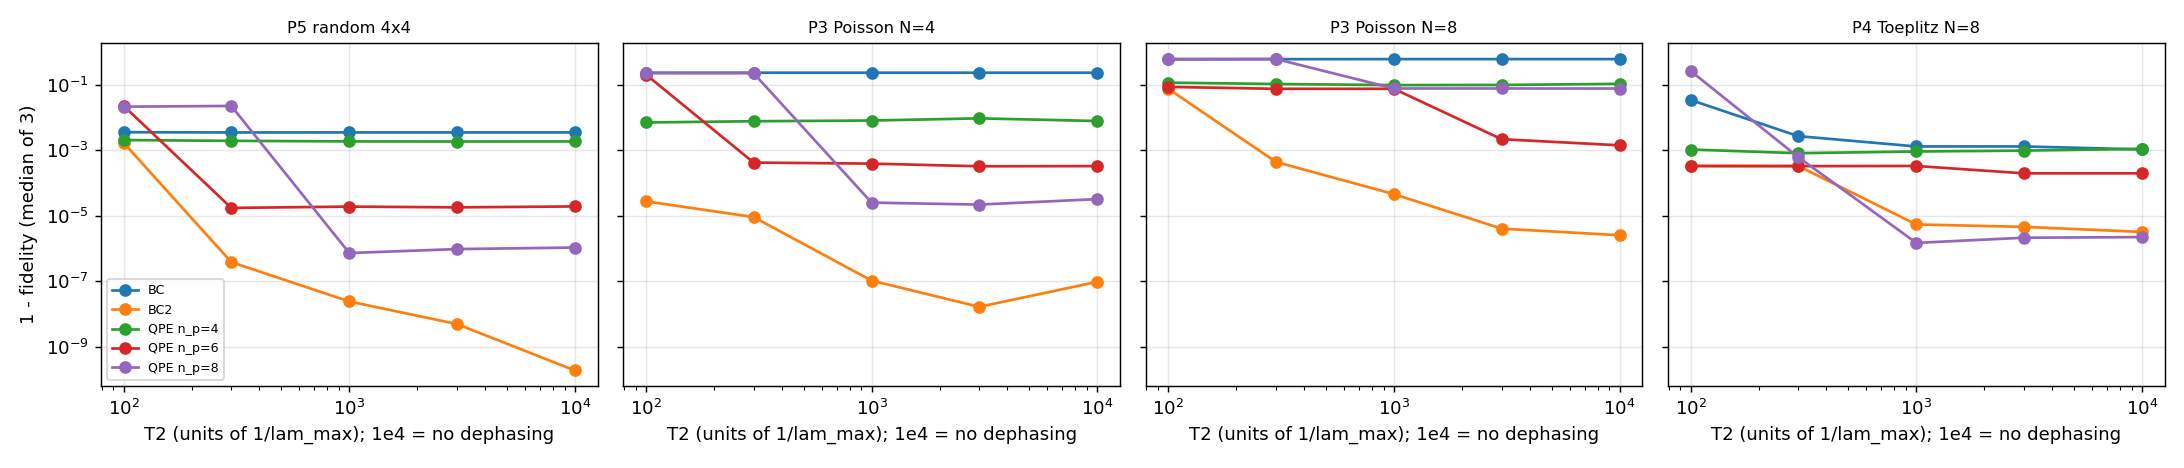
\includegraphics[width=\textwidth]{figs/fig1_T2_sweep.png}
\caption{Solution infidelity $1-F$ of the idealised hybrid solver versus the dephasing time $T_2$ (units of $1/\lmax$; $10^4$ denotes no dephasing) for the eigenvalue-learning stages, $10^4$ shots, median of three repetitions. ``BC'' is a mixture estimator (multi-level least squares), ``BC2'' the projective estimator of \eqref{eq:nc}, ``QPE $n_p$'' sampled coherent QPE with $n_p$ bits. The projective estimator stays below $10^{-3}$ for $T_2\ge300$ on all four systems, including points where eight-bit QPE (coherent time $1287$) has failed ($1-F\ge0.02$); at $T_2=100$ it reaches $1.7\times10^{-3}$ (random) and $0.075$ (Poisson $N=8$), and on Poisson $N=8$ at $T_2=300$ its distribution over 100 runs has a low group that three runs do not show (Table~\ref{tab:learn}). The mixture estimator is limited by the weak components regardless of $T_2$.}
\label{fig:T2}
\end{figure*}

\begin{table*}[t]
\caption{Median solution fidelity of the idealised hybrid solver (exact eigen-tagging, learned angles) over 100 repetitions, $10^4$ shots per run, $p_d=0.02$. Interquartile ranges are given where they exceed $0.01$. $n_c$ from \eqref{eq:nc}.}
\label{tab:learn}
\centering\footnotesize
\begin{tabular}{llcccccc}
\toprule
Problem & $T_2$ & $\kappa$ & MM-QCELS-type & QMEGS-type & QPE 6 bits & Projective ($n_c$) \\
\midrule
Random $4\times4$ & $\infty$ & 2.2 & 0.995 [0.977, 0.998] & 0.979 [0.977, 0.996] & 1.0000 & 1.0000 (5)\\
Random $4\times4$ & 300 & 2.2 & 0.998 [0.978, 0.9999] & 0.978 [0.977, 0.992] & 1.0000 & 1.0000 (5)\\
Poisson $N=4$ & $\infty$ & 9.5 & 0.941 [0.770, 0.997] & 0.889 [0.769, 0.999] & 0.9996 & 1.0000 (4)\\
Poisson $N=4$ & 300 & 9.5 & 0.968 [0.813, 0.999] & 0.818 [0.769, 0.944] & 0.999 & 1.0000 (4)\\
Poisson $N=8$ & $\infty$ & 32 & 0.880 [0.612, 0.902] & 0.757 [0.392, 0.924] & 0.999 [0.925, 0.999] & 1.0000 (5)\\
Poisson $N=8$ & 300 & 32 & 0.844 [0.394, 0.905] & 0.647 [0.430, 0.906] & 0.925 & 0.924 [0.924, 0.9997] (5)\\
Toeplitz $N=8$ & $\infty$ & 4.0 & 0.999 [0.976, 0.999] & 0.999 & 0.9998 & 1.0000 (6)\\
Toeplitz $N=8$ & 300 & 4.0 & 0.999 [0.980, 0.999] & 0.993 [0.973, 0.998] & 0.9997 & 0.9996 (5)\\
\bottomrule
\end{tabular}
\end{table*}

\begin{figure}[t!]
\centering
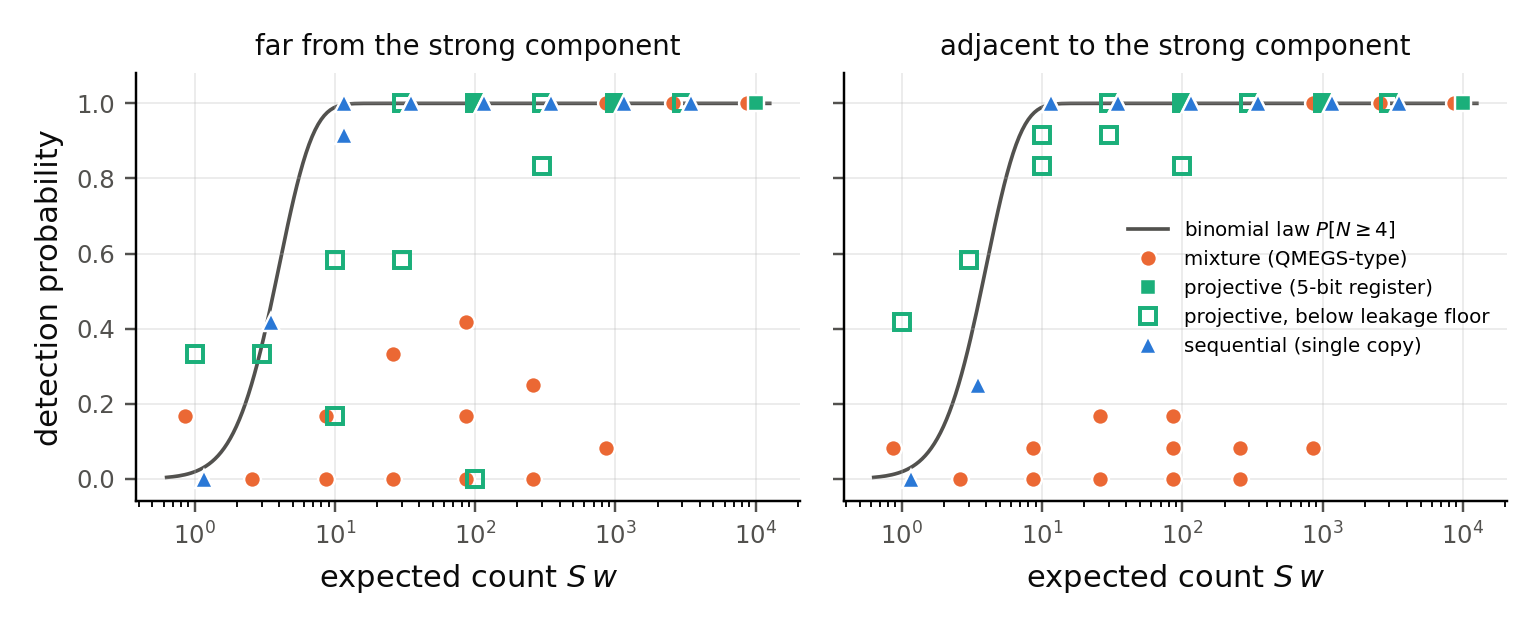
\includegraphics[width=0.98\columnwidth]{figs/fig2_detection.png}
\caption{Detection probability of a planted component of weight $w\in\{0.001,0.003,0.01,0.03,0.1\}$ (the sequential estimator up to $0.03$) in an eight-eigenvalue spectrum with one strong component ($w=0.5$), versus the expected count $Sw$ for $S\in\{10^3,10^4,10^5\}$ samples (twelve runs per point, four for the sequential estimator at $S=10^5$; markers of the three estimators are offset horizontally for visibility). Left: planted component far from the strong one; right: $1.5$ register bins from it. The sequential estimator (triangles) follows the binomial law $P[N\ge4]$ (line) at both placements and returned no false component in any run. Projective labelling with a five-bit register (squares) is hollow where the planted weight is below the leakage floor $w_{\rm fl}$ of its three bins ($0.043$ and $0.038$), where a flagged peak cannot be attributed to the planted component. The mixture estimator (QMEGS-type, circles) is not governed by $Sw$: it detects only where $w\sqrt S\gtrsim10$.\label{fig:detect}}
\end{figure}

We use four test systems with $\lmax\le1$: a random Hermitian $4\times4$ matrix with eigenvalue gaps above $0.08$, the one-dimensional Dirichlet Poisson matrix for $N=4$ and $N=8$ ($\kappa=9.5$ and $32$), and a diagonally dominant symmetric Toeplitz matrix for $N=8$ whose smallest gap is $0.0034$; $|b\rangle$ is a random unit vector in each case, so that weak components ($w_j$ down to $10^{-3}$) occur. All measurement statistics are sampled exactly from \eqref{eq:p} (and from the corresponding clock amplitudes for QPE, with Gaussian phase kicks of variance $2\cdot2^kt_0/T_2$ on each controlled $U^{2^k}$), with $10^4$ shots per learning run. Fidelity is first evaluated for the idealised solver in which eigen-tagging is exact and only the rotation angles come from the learned values, so that the learning stages are compared in isolation.

Fig.~\ref{fig:T2} and Table~\ref{tab:learn} show the result. The mixture estimators are limited by the weak components, as \eqref{eq:prop} predicts: on Poisson $N=8$, whose weights are $0.032$ and $0.006$ at the two smallest eigenvalues ($\lambda=0.031$ and $0.121$) and $0.001$ at the fifth, their median fidelity is $0.76$--$0.88$ without dephasing and they reach $F\ge0.99$ in $1$ (MM-QCELS-type) and $13$ (QMEGS-type) of the 100 runs; the QMEGS-type runs form several groups there ($26$ at $0.38$--$0.40$, $21$ at $0.92$--$0.93$, $13$ at $F\ge0.99$), and the medians of the first and of the second fifty runs are $0.91$ and $0.54$, so its median is not a stable summary. The detection runs in Appendix~\ref{app:proofs} and the mixture points of Fig.~\ref{fig:detect} show the mechanism: at $10^4$ shots both mixture estimators miss all three components, whose amplitudes are below the per-point noise $1/\sqrt{S_{\rm pt}}\approx0.12$ of the time series; at $10^5$ shots the QMEGS-type estimator finds the $w=0.032$ component in every run and reaches $F=0.92$--$0.99$, while the MM-QCELS-type estimator still misses it in two of three runs, which is a limitation of that implementation rather than of the data.

Sampled six-bit QPE and the projective estimator both reach a median $F\ge0.998$ in every case without dephasing, but not with the same reliability: on Poisson $N=8$ six-bit QPE falls to $0.925$ in $32$ of the 100 runs, whereas the projective estimator stays above $0.97$ in all of them. The two also differ in resources. Under dephasing the difference is in the coherent time (Fig.~\ref{fig:T2}, medians of three runs). Eight-bit QPE (coherent time $1287$) falls to $1-F\ge0.02$ at $T_2\le300$ on the random and Poisson $N=4$ systems and at $T_2=100$ on the Toeplitz system, and six-bit QPE (coherent time $322$) at $T_2=100$ on the random and Poisson $N=4$ systems; elsewhere on these three systems both stay below $10^{-3}$. On Poisson $N=8$ both are limited before dephasing matters: in two of the three runs without dephasing eight-bit QPE does not select the $\lambda=0.121$ component, because side lobes of the strong component at $\lambda=0.773$ collect more counts, and its median stays at $1-F=0.076$--$0.077$ for $T_2\ge1000$; six-bit QPE is at $0.075$--$0.086$ for $T_2\le1000$.

The labelled estimator with $n_c=4$--$5$ (coherent time $80$--$160$) keeps a median $F\ge0.9996$ at $T_2=300$ on three systems and degrades at $T_2=100$ (to $0.998$ on the random system and $0.92$ on Poisson $N=8$); on Poisson $N=8$ at $T_2=300$ its runs form two groups, median $0.924$ with upper quartile $0.9997$: $57$ of the 100 runs are below $0.93$. In $55$ of them ($F=0.92$--$0.93$) the dephased coarse clock does not resolve the $w=0.006$ component at $\lambda=0.121$ ($q=0.011$), and the solver rotates it with the learned value of $\lambda=0.031$, which costs $0.076$ by the exact expression after \eqref{eq:prop} ($0.09$ to leading order); in the other two ($F=0.84$ and $0.86$) the $\lambda=0.031$ component itself is learned at $0.077$. None of the $43$ runs above $0.93$ shows the merger, and the seven low runs of Table~\ref{tab:matched} all do. The $32$ low runs of six-bit QPE without dephasing and all 100 at $T_2=300$ show the same merger, which is why the two estimators have the same median at $T_2=300$. The other low tails of the projective estimator are small: $6$ of 100 runs below $0.99$ on Poisson $N=4$ at $T_2=300$ (minimum $0.969$) and $3$ of 100 on Poisson $N=8$ without dephasing (minimum $0.972$). This is the leakage floor of Sec.~\ref{sec:stages}, raised by dephasing, and not a shot-count effect.

The refinement time cap does not change this in the range tested (in separate sets of 100 runs that use the same random numbers for every cap between $0.5T_2$ and $3T_2$, the median is $0.924$--$0.925$, the quartiles are $0.924$ and $0.999$, $60$ or $61$ runs are below $0.93$, and one run changes group; without dephasing the result is unchanged when the refinement is capped at $2000$, the window of the mixture baselines), so under dephasing the coherent coarse stage, not the incoherent refinement, is the limiting element.

Table~\ref{tab:learn} compares whole estimators at the same number of shots, each with its own time rule, and not at equal evolution time: the refinement of the projective estimator is capped at $2T_2$ ($2000$ without dephasing), the MM-QCELS-type time grid extends to $295$ at $T_2=300$ and to $2359$ without dephasing, the QMEGS-type estimator draws $|t|$ from a Gaussian of width $T=\min(T_2,2000)$, so that $32\%$ of its times exceed $T$, and six-bit QPE has a coherent window of $322$; coarse registers have at most six bits. The sequential estimator of Sec.~\ref{sec:stages} is compared with the projective one separately, within the same budget of total evolution time, in the next subsection.

\begin{table*}[t]
\caption{Identification cost of one copy, $c_{\rm id}=T_{\rm id}\sigma_{\rm id}$ (mean), and fraction of estimates farther than $3\sigma_{\rm id}$ and $4\sigma_{\rm id}$ from the eigenvalue, versus the stopping threshold $p_{\rm out}$, for a flat prior and for the prior learned by a preceding run of the estimator ($5\times10^6$ time units; all eight components found). ``Exact'': the true spectrum as prior, for reference. Poisson $N=8$, $\sigma_{\rm id}=0.0112$, $24\,000$ copies per entry, matched contrast. With zero events in $24\,000$ copies the one-sided $95\%$ upper limit on the fraction is $1.2\times10^{-4}$.}
\label{tab:cost}
\centering\footnotesize
\begin{tabular}{lccccccccc}
\toprule
 & \multicolumn{3}{c}{flat prior} & \multicolumn{3}{c}{learned prior} & exact & \multicolumn{2}{c}{$T_2=300$}\\
$p_{\rm out}$ & $c_{\rm id}$ & $>3\sigma_{\rm id}$ & $>4\sigma_{\rm id}$ & $c_{\rm id}$ & $>3\sigma_{\rm id}$ & $>4\sigma_{\rm id}$ & $c_{\rm id}$ & $c_{\rm id}$ flat & $c_{\rm id}$ learned\\
\midrule
$10^{-2}$ & 5.5 & 2.0e-3 & 1.0e-3 & 1.3 & 3.3e-4 & 3.3e-4 & 1.2 & 7.0 & 1.5\\
$10^{-3}$ & 6.5 & 2.1e-4 & 8.3e-5 & 2.7 & 0 & 0 & 2.6 & 8.3 & 3.3\\
$10^{-4}$ & 8.8 & 1.7e-4 & 0 & 5.0 & 0 & 0 & 4.5 & 11.8 & 6.4\\
$10^{-5}$ & 11.6 & 0 & 0 & 8.0 & 0 & 0 & 6.9 & 16.2 & 10.0\\
\bottomrule
\end{tabular}
\end{table*}

\begin{table}[t]
\caption{Fraction of estimates farther than $3\sigma_{\rm id}$ and $4\sigma_{\rm id}$ from the eigenvalue when the contrast assumed by the estimator differs from the true one (assumed $\to$ true; ``matched'': no mismatch). Flat prior, Poisson $N=8$, $24\,000$ copies per entry.}
\label{tab:miscal}
\centering\footnotesize
\begin{tabular}{lcccc}
\toprule
 & \multicolumn{2}{c}{$p_{\rm out}=10^{-3}$} & \multicolumn{2}{c}{$p_{\rm out}=10^{-4}$}\\
contrast & $>3\sigma_{\rm id}$ & $>4\sigma_{\rm id}$ & $>3\sigma_{\rm id}$ & $>4\sigma_{\rm id}$\\
\midrule
$T_2=300$, matched & 4.6e-4 & 4.2e-5 & 0 & 0\\
$T_2$: $300\to100$ & 8.3e-3 & 2.6e-3 & 4.2e-4 & 4.2e-5\\
no dephasing, matched & 2.1e-4 & 8.3e-5 & 1.7e-4 & 0\\
$p_d$: $0.02\to0.10$ & 2.6e-3 & 1.2e-3 & 2.9e-4 & 4.2e-5\\
$p_d$: $0.02\to0.20$ & 8.7e-3 & 4.3e-3 & 1.7e-3 & 6.7e-4\\
$T_2$: $\infty\to1000$ & 7.9e-4 & 1.7e-4 & 1.3e-4 & 0\\
\bottomrule
\end{tabular}
\end{table}

\begin{table*}[t]
\caption{Solution infidelity $1-F$ of the idealised hybrid solver for four labelled estimators within the same budget of total evolution time $T_{\rm tot}$, the median time of the ten projective runs with $10^4$ shots (units of $1/\lmax$; individual projective runs use $0.58$--$1.03\,T_{\rm tot}$, the other three estimators never more than $T_{\rm tot}$); median and worst of ten independent repetitions (no common random numbers between estimators), entries written as $2.8\mathrm{e}{-6}=2.8\times10^{-6}$. ``Projective'': register label and one refinement measurement on every shot. ``Proj., target'': the same with the refinement stopped once a component reaches the relative precision $\delta=10^{-3}$, with the largest number of shots that fits into $T_{\rm tot}$. ``Seq., every copy'': sequential estimator with one refinement measurement on every copy. ``Seq., target'': refinement stopped at $\delta=10^{-3}$ (or $10^{-4}$); $\hat m$ is the median number of components found (the projective estimator is given $m$), and the last column uses $T_{\rm tot}/10$. The sequential estimator never exceeds its time budget. $\sigma_{\rm id}=\Delta_{\min}/8$, except Toeplitz, where $\sigma_{\rm id}=0.005$, a quarter of a six-bit bin.}
\label{tab:matched}
\centering\footnotesize
\begin{tabular}{llcccccccccccc}
\toprule
 & & & \multicolumn{2}{c}{Projective} & \multicolumn{2}{c}{Proj., target} & \multicolumn{2}{c}{Seq., every copy} & \multicolumn{3}{c}{Seq., target $10^{-3}$} & $10^{-4}$ & $T_{\rm tot}/10$\\
Problem & $T_2$ & $T_{\rm tot}$ & med. & worst & med. & worst & med. & worst & med. & worst & $\hat m$ & med. & med.\\
\midrule
Random $4\times4$ & $\infty$ & 2.0e7 & 7.4e-10 & 5.2e-9 & 6.3e-7 & 1.5e-6 & 3.2e-10 & 1.7e-9 & 4.3e-7 & 9.8e-7 & 4 & 3.6e-9 & 5.8e-7\\
Random $4\times4$ & 300 & 4.1e6 & 2.1e-6 & 1.2e-5 & 1.4e-6 & 1.6e-5 & 3.7e-7 & 5.2e-6 & 4.5e-7 & 8.2e-7 & 4 & 7.7e-8 & 7.8e-7\\
Poisson $N=4$ & $\infty$ & 2.0e7 & 8.1e-8 & 2.3e-7 & 4.4e-7 & 1.4e-6 & 5.4e-9 & 3.0e-8 & 2.3e-7 & 8.8e-7 & 4 & 5.5e-9 & 2.3e-7\\
Poisson $N=4$ & 300 & 3.5e6 & 3.9e-5 & 2.7e-3 & 2.1e-5 & 8.7e-3 & 2.2e-6 & 1.2e-5 & 5.8e-7 & 1.4e-6 & 4 & 2.4e-6 & 5.2e-5\\
Poisson $N=8$ & $\infty$ & 2.0e7 & 2.8e-6 & 1.8e-4 & 2.7e-6 & 1.3e-3 & 6.8e-8 & 8.9e-6 & 8.8e-8 & 5.4e-7 & 8 & 7.8e-9 & 2.4e-6\\
Poisson $N=8$ & 300 & 4.2e6 & 0.076 & 0.076 & 0.013 & 0.076 & 2.6e-5 & 2.9e-4 & 5.8e-6 & 1.9e-5 & 7 & 1.0e-4 & 0.076\\
Toeplitz $N=8$ & $\infty$ & 2.2e7 & 4.4e-6 & 5.7e-6 & 3.6e-6 & 3.5e-4 & 4.9e-7 & 2.3e-6 & 1.3e-6 & 4.7e-6 & 7 & 4.8e-7 & 4.1e-6\\
Toeplitz $N=8$ & 300 & 4.2e6 & 3.9e-4 & 5.8e-4 & 5.2e-4 & 1.0e-3 & 3.2e-6 & 5.6e-6 & 3.0e-6 & 6.6e-6 & 6 & 5.6e-6 & 8.7e-4\\
\bottomrule
\end{tabular}
\end{table*}

\begin{table*}[t]
\caption{Relative error of the compliance (median of ten repetitions) and number of samples for the runs of Table~\ref{tab:matched}; the projective estimator uses $10^4$ shots.}
\label{tab:matchedC}
\centering\footnotesize
\begin{tabular}{llccccccc}
\toprule
 & & \multicolumn{4}{c}{compliance error (\%)} & \multicolumn{3}{c}{samples}\\
Problem & $T_2$ & Proj. & Proj., target & Seq., every & Seq., target & Proj., target & Seq., every & Seq., target\\
\midrule
Random $4\times4$ & $\infty$ & 0.09 & 0.14 & 0.15 & 0.09 & 128125 & 8504 & 50542\\
Random $4\times4$ & 300 & 0.15 & 0.21 & 0.30 & 0.20 & 23945 & 4600 & 6452\\
Poisson $N=4$ & $\infty$ & 0.23 & 0.18 & 0.35 & 0.17 & 261250 & 9507 & 136761\\
Poisson $N=4$ & 300 & 0.61 & 0.61 & 0.63 & 0.22 & 34375 & 7437 & 8326\\
Poisson $N=8$ & $\infty$ & 1.7 & 0.35 & 1.9 & 0.86 & 125625 & 8554 & 48166\\
Poisson $N=8$ & 300 & 2.9 & 1.8 & 2.4 & 1.7 & 20351 & 4644 & 4312\\
Toeplitz $N=8$ & $\infty$ & 0.46 & 0.55 & 0.72 & 0.20 & 70000 & 7222 & 20910\\
Toeplitz $N=8$ & 300 & 0.67 & 1.0 & 0.82 & 0.51 & 20624 & 1955 & 1718\\
\bottomrule
\end{tabular}
\end{table*}

\subsection{Recycled sequential HHL}

Table~\ref{tab:cost} gives the cost and the error of the identification. At $p_{\rm out}=10^{-4}$ a copy costs $8.8/\sigma_{\rm id}$ from a flat prior and $5.0/\sigma_{\rm id}$ with the learned prior ($11.8$ and $6.4$ at $T_2=300$); with the exact spectrum as prior it would cost $4.5/\sigma_{\rm id}$. The fraction of estimates farther than $3\sigma_{\rm id}$ from the eigenvalue, the event the stopping rule refers to, does not exceed $p_{\rm out}$ in seven of the eight entries (two of them, at $p_{\rm out}=10^{-5}$, have no event, which $24\,000$ copies cannot distinguish from $10^{-5}$) and is $1.7\times10^{-4}$ in the eighth (flat prior, $p_{\rm out}=10^{-4}$); no estimate is farther than $4\sigma_{\rm id}$ for $p_{\rm out}\le10^{-4}$, which with $24\,000$ copies bounds that fraction only at the $10^{-4}$ level. Lowering $p_{\rm out}$ by a factor of ten adds between $1.0$ and $3.0$ to $c_{\rm id}$ without dephasing and between $1.3$ and $4.5$ at $T_2=300$, the increments growing as $p_{\rm out}$ falls. The threshold is not robust to a wrong noise model (Table~\ref{tab:miscal}): when the contrast is over-estimated, by a dephasing time three times too long or a depolarising rate five to ten times too small, the fraction beyond $3\sigma_{\rm id}$ rises to as much as $9$ times $p_{\rm out}$ at $p_{\rm out}=10^{-3}$ and $17$ times at $p_{\rm out}=10^{-4}$, whereas a weak unmodelled dephasing ($T_2=1000$ instead of none) leaves it near $p_{\rm out}$. The degradation is gradual, and it is still far below the $1/(\pi^2d^2)$ tail of a register, but $p_{\rm out}$ must be read as a design parameter whose effect has to be measured.

Fig.~\ref{fig:detect} shows the consequence for detection. With planted weights between $10^{-3}$ and $0.03$ the sequential estimator detects the component with the binomial probability of collecting four copies: $0.25$--$0.42$ at $Sw=3$, $0.92$--$1$ at $Sw=10$ and $1$ above, far from and next to the strong component alike, and it returned no false component in any run up to $10^5$ copies. The projective estimator does not find $w=0.001$ far from the strong component even with $10^5$ shots, and next to the strong component its detections below $w\approx0.04$ are under the leakage floor. A copy costs $3.3$--$4.2$ register shots in this test once the prior is learned ($6$--$8$ in the first $10^3$ copies); more register shots do not lower the floor.

Table~\ref{tab:matched} compares four labelled estimators within the same budget of total evolution time: the projective and the sequential estimator, each with a refinement measurement on every sample and with the refinement stopped at a precision target. The budget $T_{\rm tot}$ is the median time of the ten projective runs with $10^4$ shots, whose individual times are $0.58$--$1.03\,T_{\rm tot}$; the projective estimator with the target uses the largest number of shots that fits ($0.86$--$1.00\,T_{\rm tot}$), and the sequential estimator stops at $T_{\rm tot}$.

With a refinement on every sample, the sequential estimator has the lower median infidelity on all eight system and noise combinations, by factors between $2.3$ (random system, no dephasing) and $2.9\times10^3$ (Poisson $N=8$, $T_2=300$); on Poisson $N=8$ without dephasing the median falls from $2.8\times10^{-6}$ to $6.8\times10^{-8}$, and at $T_2=300$, where the dephased coarse register does not resolve the $w=0.006$ component at $\lambda=0.121$ in seven of these ten runs ($55$ of 100 in the independent runs of Table~\ref{tab:learn}), so that it is rotated with $\lambda=0.031$ and the projective estimator stays at $0.076$, to $2.6\times10^{-5}$. With the target on both it is lower on all eight as well, by factors of $1.5$ to $2.2\times10^3$. The advantage thus persists under both allocation policies, and giving the projective estimator the target does not remove its failure on Poisson $N=8$ ($2.7\times10^{-6}$ without dephasing; median $0.013$ and worst run $0.076$ at $T_2=300$), which is consistent with its eigenvalues being limited by the purity of the register label and by the unresolved (merged) component. The allocation is not without effect: it changes the medians of both estimators on the other systems, and the four columns compare whole estimators, not the label in isolation. The worst runs of the projective estimator with the target reach $1.3\times10^{-3}$ (Poisson $N=8$, no dephasing) and $8.7\times10^{-3}$ (Poisson $N=4$, $T_2=300$).

All eight components of Poisson $N=8$ are found without the number being supplied when there is no dephasing, and seven at $T_2=300$. On the Toeplitz system, $\sigma_{\rm id}=0.005$ separates the pair at $\lambda=0.921$ and $0.938$ (weights $0.023$ and $0.80$), which the six-bit register does not resolve, in all ten runs without dephasing and in seven of ten at $T_2=300$, and leaves the pair $0.0034$ apart merged ($\hat m=7$); resolving that pair needs $\sigma_{\rm id}=4\times10^{-4}$. Every copy is then identified at that resolution and the same time buys $5.1\times10^3$ copies instead of $2.1\times10^4$; all eight components are found and the median infidelity is $1.2\times10^{-7}$ against $1.3\times10^{-6}$ (five repetitions), but a tenth of the time runs only $400$ copies and finds six. A resolution that is refined only where estimates cluster would avoid this cost and is not implemented.

The estimator fails when the time does not cover both identification and the refinement of the dominant component. With $T_{\rm tot}/10$ on Poisson $N=8$ at $T_2=300$ only $160$ copies are run and the median infidelity is $0.076$ (worst $0.61$); on the Toeplitz system at $T_2=300$ the same fraction gives $8.7\times10^{-4}$ (worst $0.034$, four components found). With $\delta=10^{-4}$ and $T_{\rm tot}/10$ on Poisson $N=8$ without dephasing the refinement of the first components exhausts the time and the median is again $0.076$; and with $\delta=10^{-4}$ at $T_2=300$ the median is $1.0\times10^{-4}$ and the worst run $0.076$. The target must be set from the time available, as is done for observables in Sec.~\ref{sec:solver}.

For the weights the picture is different (Table~\ref{tab:matchedC}): neither labelled estimator is uniformly better. A register label is cheaper than a sequential copy, $156$ against about $420$ time units on Poisson $N=8$, so that the projective estimator with the target collects $1.3\times10^5$ shots where the sequential one collects $4.8\times10^4$ copies, and its compliance error is the smaller there ($0.35\%$ against $0.86\%$). More shots do not, however, systematically lower the projective error: with the target it has $2$ to $26$ times as many shots as without, and its compliance error falls in three of the eight combinations and does not in five, so that it is not limited by sampling there. The sequential error is lower with the target than without on all eight. Over the eight combinations the smallest error belongs to the sequential estimator with the target in six (two of them near-ties), to the projective estimator in one and to the projective estimator with the target in one; with ten repetitions the ranking should not be over-read. Averaged over a run, a sequential copy costs $1.9$ to $3.4$ times a register label without dephasing and $4$ to $16$ times at $T_2=300$. In the two main sequential columns of Table~\ref{tab:matched} (every copy; target $\delta=10^{-3}$) every copy converged and at most $0.3\%$ of the copies were left without a label; with $\delta=10^{-4}$ up to $0.7\%$ are, with $T_{\rm tot}/10$ up to $6\%$, and in the smallest runs of the other settings, with fewer than a hundred copies, up to $23\%$.

Equation~\eqref{eq:record} assumes that the system register is disturbed only by the measurements. As a first test we let the copy lose its eigencomponent at a rate $1/T_{\rm sys}$, redrawing it with probabilities $w_j$ (Poisson $N=8$, no dephasing, $T_{\rm tot}=2\times10^6$, $\delta=10^{-3}$). The median infidelity stays between $2.4\times10^{-6}$ and $5.0\times10^{-6}$ for $T_{\rm sys}\ge3\times10^4$ (worst run $1.7\times10^{-5}$) and rises to $3.1\times10^{-5}$ at $T_{\rm sys}=10^4$, where the worst of ten runs is $0.021$; no false component appeared, and seven of the eight components were found throughout. A copy lives for up to about $4\times10^4$ time units in the runs with a target and for $9\times10^2$ to $1\times10^4$ with one refinement per copy, against about $2\times10^3$ for a projective shot. Section~\ref{sec:system} extends this test to a depolarised register and to two of the application problems.

\section{The learning stage as a solver}
\label{sec:solver}

\begin{table*}[t]
\caption{Observable-first solver (projective estimator, median of six repetitions, the runs of Table~\ref{tab:qoiseq}) versus two model-free estimators built from the same controlled-$e^{-iAt}$ Hadamard tests (median of four repetitions): a time-evolution quantum Krylov solver (QKS, projected matrices from $g(t)$ and $h(t)=\langle b|Ae^{-iAt}|b\rangle$, thresholded regularisation, best of a small grid of subspace sizes) and the randomised Fourier representation of $A^{-1}$ (truncation $Y=\kappa\log10^3$). Relative errors of the compliance $C=\langle b|A^{-1}|b\rangle$, the energy ratio $E=\langle x|A|x\rangle/\langle x|x\rangle$ and a linear functional $L=\langle v|A^{-1}|b\rangle$ with a random unit $v$, for total budgets of $10^4$ and $1.6\times10^5$ shots split over the four input states.}
\label{tab:qoi}
\centering\footnotesize
\begin{tabular}{llccccc}
\toprule
Problem & $T_2$ & \multicolumn{2}{c}{Spectral: $C$ / $E$ / $L$} & \multicolumn{2}{c}{QKS: $C$ / $E$ / $L$} & Fourier: $L$\\
 & & $10^4$ & $1.6\times10^5$ & $10^4$ & $1.6\times10^5$ & $10^4$ / $1.6\times10^5$\\
\midrule
Random $4\times4$ & $\infty$ & 0.31 / 0.36 / 3.0\% & 0.09 / 0.11 / 1.0\% & 3.5 / 12 / 51\% & 1.5 / 2.4 / 15\% & 168 / 40\%\\
Random $4\times4$ & 300 & 0.54 / 0.94 / 4.6\% & 0.14 / 0.23 / 2.1\% & 19 / 27 / 81\% & 3.3 / 2.7 / 27\% & 131 / 44\%\\
Poisson $N=4$ & $\infty$ & 1.7 / 2.6 / 3.4\% & 0.45 / 0.46 / 1.6\% & 41 / 61 / 43\% & 9.2 / 6.6 / 17\% & 102 / 16\%\\
Poisson $N=4$ & 300 & 0.94 / 1.8 / 6.5\% & 0.33 / 0.62 / 1.6\% & 15 / 31 / 38\% & 8.1 / 18 / 14\% & 142 / 22\%\\
Poisson $N=8$ & $\infty$ & 1.4 / 2.8 / 11\% & 0.84 / 1.1 / 2.5\% & 29 / 459 / 71\% & 25 / 301 / 56\% & 584 / 157\%\\
Poisson $N=8$ & 300 & 8.3 / 14 / 12\% & 2.9 / 4.9 / 4.4\% & 38 / 302 / 81\% & 21 / 177 / 59\% & 923 / 445\%\\
Toeplitz $N=8$ & $\infty$ & 1.1 / 1.0 / 48\% & 0.76 / 1.1 / 48\% & 57 / 62 / 283\% & 9.8 / 18 / 95\% & 451 / 117\%\\
Toeplitz $N=8$ & 300 & 0.66 / 1.6 / 47\% & 0.81 / 0.47 / 50\% & 73 / 61 / 256\% & 3.2 / 8.8 / 142\% & 728 / 128\%\\
\bottomrule
\end{tabular}
\end{table*}

The projective estimator returns, for each learned eigenvalue, a label count. Solving the non-negative least-squares problem $\mathrm{counts}(y)/S\approx\sum_j\hat w_jP_j(y)$ with the (dephasing-averaged) clock kernel $P_j$ computed from the learned $\mu_j$ gives the weights $\hat w_j$; reading them directly from the $\pm1$ bins would be biased by the $19\%$ leakage. The pair $\{(\mu_j,\hat w_j)\}$ is the spectral measure of $A$ on $|b\rangle$, and for any $f$ that is $C^1$ on $[\lmin,1]$,
\begin{align}
\Big|\sum_j\hat w_jf(\mu_j)-\langle b|f(A)|b\rangle\Big|\le{}&\sum_j\big(|\eta_j||f(\lambda_j)|\nonumber\\
&+\hat w_j|f'(\xi_j)||\delta_j|\big),
\label{eq:qoi}
\end{align}
with $\eta_j=\hat w_j-w_j$. The compliance ($f=1/\lambda$), the energy ratio and the eigenmode weights of the solution follow without any further quantum circuit. Linear functionals need the cross weights $c_j=\langle v|u_j\rangle\langle u_j|b\rangle$, which the polarisation identity $c_j=\tfrac12(w^{(b+v)}_j\|b+v\|^2-w_j-w^{(v)}_j)+\tfrac i2(w^{(b+iv)}_j\|b+iv\|^2-w_j-w^{(v)}_j)$ obtains from the diagonal weights of four input states, learned with the eigenvalue set fixed by the $|b\rangle$ run. When the refinement has made the eigenvalue errors subdominant, \eqref{eq:qoi} is dominated by the weight errors $\eta_j\sim\sqrt{w_j/S}$ times the conditioning of the kernel, and the shot cost of the observable-first solver follows the sampling law $1/\varepsilon^2$.

Two model-free references use exactly the same primitive. The first is time-evolution quantum Krylov linear solving \cite{YuZhou2026,Park2026}: the states $e^{-iAt_k}|b\rangle$ span a subspace whose overlap and projected matrices are $S_{kl}=g(t_l-t_k)$ and $H_{kl}=h(t_l-t_k)$ with $h(t)=\langle b|Ae^{-iAt}|b\rangle$ (one controlled application of $A$ per Hadamard test), the projected system $Hc=r$ is solved after thresholding the small eigenvalues of $S$, and the observables follow from $c$ and the same polarised Hadamard tests. Its input data are the mixture functions $g$ and $h$, so the weights of weak components enter with the mixture detection law, and the thresholded inversion of an ill-conditioned overlap matrix amplifies shot noise; the implementation used here is the plain thresholded variant and does not include the directional-stability constructions of \cite{YuZhou2026}, so its numbers bound that variant only. The second is the randomised Fourier representation $A^{-1}=i\int_0^\infty dy\,\mathbb E_{z\sim\mathcal N(0,1)}[z\,e^{-iyzA}]$, truncated at $y\le Y=\kappa\log(1/\varepsilon)$ and sampled one $(y,z)$ per Hadamard test, which is unbiased up to the truncation but has variance $\sim Y^2/S$ and hence a shot cost $\propto\kappa^2\log^2(1/\varepsilon)/\varepsilon^2$ \cite{Hariprakash2025}.

Table~\ref{tab:qoi} shows the outcome. With $10^4$ shots the spectral-measure solver returns the compliance and the energy to $0.3$--$2.8\%$ on all four systems without dephasing; under $T_2=300$ the Poisson $N=8$ errors rise to $8$--$14\%$, while the other systems stay below $2\%$; the eigenvalue term of \eqref{eq:qoi} at the smallest eigenvalues, the weight error of the kernel inversion and the unresolved $\lambda=0.121$ component of Table~\ref{tab:matched} can all contribute there, and their shares were not separated. Linear functionals are harder: the cross weights $c_j$ alternate in sign on the Toeplitz system, on which two pairs of eigenvalues are closer than one six-bit bin ($0.414$ and $0.417$; $0.921$ and $0.938$, the latter with weights $0.023$ and $0.80$) and are merged into clusters, and the relative error stays near $48\%$ at both budgets, which is consistent with a cancellation between merged components; on the other three systems $1.0$--$4.4\%$ is reached with $1.6\times10^5$ shots. The thresholded Krylov solver, with the same data and shots, is worse by factors of $2$ to $280$ and does not improve monotonically with shots; the Fourier estimator is worse by factors of $2.5$ to $100$ and would need of order $10^8$ shots at evolution times near $750$ for a $1\%$ compliance on Poisson $N=8$.

A statement that does not depend on the post-processing, within its class of estimators, is the Cram\'er--Rao bound for a given measurement design: a lower bound on the standard deviation of locally unbiased estimators. For the compliance it must be taken jointly over the weights on the simplex, since errors of different weights can cancel in $C$ (Appendix~\ref{app:proofs}). On Poisson $N=8$ with $10^4$ mixture shots and known eigenvalues the bound on the relative standard deviation is $13\%$ for random evolution times of the kind used by the mixture baselines (Gaussian windows from $30$ to $2000$) and about $6\%$ for the best design found on a grid of settings. These are not bounds on the median errors of Table~\ref{tab:qoi}, nor on biased or regularised estimators, and an estimate from the approximate cumulative distribution function of \cite{LinTong2022} may use another design and is not implemented here; they indicate the scale at which mixture data constrain $C$, which is four to nine times the $1.4\%$ median error of the labelled estimate (Table~\ref{tab:qoi}). The Krylov and Fourier errors are above this scale, so they should be read as what the plain variants achieve rather than as the best mixture post-processing.

The comparison fixes the regime of the observable-first solver: few weighted components ($m$ small, $w_{\min}$ not small), where learning the measure costs $O(w_{\min}^{-1})$ samples for detection, a refinement time that grows as $1/\varepsilon$ without a cap on the evolution time and as $1/\varepsilon^2$ with one, and $O(1/\varepsilon^2)$ samples for the weights; when $m$ grows with the dimension the model-free estimators, or the coherent solvers, take over.

\begin{table*}[t]
\caption{Observables from the learned measure within the same budget of total evolution time: projective estimator (weights from the kernel inversion) and sequential estimator (weights from label frequencies, refinement target set from the sensitivity of $C$). Relative errors of $C$ / $E$ / $L$, median of six independent repetitions each; the budget of the sequential estimator is the median time of the six projective runs with $10^4$ and $1.6\times10^5$ shots, measured on those runs (which individually use $0.78$--$1.02$ of it), and is not exceeded.}
\label{tab:qoiseq}
\centering\footnotesize
\begin{tabular}{llcccc}
\toprule
 & & \multicolumn{2}{c}{time of $10^4$ shots} & \multicolumn{2}{c}{time of $1.6\times10^5$ shots}\\
Problem & $T_2$ & Projective & Sequential & Projective & Sequential\\
\midrule
Random $4\times4$ & $\infty$ & 0.31 / 0.36 / 3.0\% & 0.23 / 0.40 / 2.3\% & 0.09 / 0.11 / 1.0\% & 0.08 / 0.08 / 0.54\%\\
Random $4\times4$ & 300 & 0.54 / 0.94 / 4.6\% & 0.59 / 0.75 / 4.9\% & 0.14 / 0.23 / 2.1\% & 0.15 / 0.17 / 0.60\%\\
Poisson $N=4$ & $\infty$ & 1.7 / 2.6 / 3.4\% & 0.35 / 0.54 / 1.7\% & 0.45 / 0.46 / 1.6\% & 0.12 / 0.23 / 0.49\%\\
Poisson $N=4$ & 300 & 0.94 / 1.8 / 6.5\% & 1.0 / 2.7 / 2.4\% & 0.33 / 0.62 / 1.6\% & 0.22 / 0.70 / 1.3\%\\
Poisson $N=8$ & $\infty$ & 1.4 / 2.8 / 11\% & 2.4 / 2.5 / 7.6\% & 0.84 / 1.1 / 2.5\% & 0.59 / 1.2 / 1.4\%\\
Poisson $N=8$ & 300 & 8.3 / 14 / 12\% & 8.5 / 15 / 12\% & 2.9 / 4.9 / 4.4\% & 2.9 / 4.8 / 3.0\%\\
Toeplitz $N=8$ & $\infty$ & 1.1 / 1.0 / 48\% & 0.82 / 0.81 / 8.6\% & 0.76 / 1.1 / 48\% & 0.32 / 0.57 / 2.5\%\\
Toeplitz $N=8$ & 300 & 0.66 / 1.6 / 47\% & 2.5 / 4.2 / 24\% & 0.81 / 0.47 / 50\% & 0.64 / 1.4 / 8.4\%\\
\bottomrule
\end{tabular}
\end{table*}

With the sequential estimator the weights are label frequencies, $\hat w_j=N_j/S$. If the labels were exact, the counts multinomial with fixed $S$, and the eigenvalue errors unbiased and independent of each other and of the counts, then
\begin{equation}
\mathrm{Var}\,\hat C=\frac VS+\sum_j\frac{w_j^2}{\lambda_j^2}\,\mathbb E[e_j^2],\quad V=\sum_j\frac{w_j}{\lambda_j^2}-C^2,
\label{eq:multinom}
\end{equation}
to first order. The implemented estimator shares copies between identification, clustering and refinement, so \eqref{eq:multinom} is a model and not a derived property. The coefficient $\sqrt V/C$ of $1/\sqrt S$ in the relative error is $0.21$, $0.69$, $2.0$ and $0.63$ for the random, Poisson $N=4$, Poisson $N=8$ and Toeplitz inputs. In the runs of Table~\ref{tab:matchedC} with the target $\delta=10^{-3}$ the measured median compliance error is $0.86\%$ with $4.8\times10^4$ copies on Poisson $N=8$, where the first term of \eqref{eq:multinom} predicts a median of $0.61\%$, and $0.09\%$ with $5.1\times10^4$ copies on the random system, where it predicts $0.06\%$: the model gives the scale, within a factor of $1.5$. For observables we use it to set the refinement target, as a heuristic: each component is refined until its eigenvalue term is a quarter of its $1/\hat m$ share of the first term, and no further.

Table~\ref{tab:qoiseq} compares the two labelled estimators on the three observables, with the projective estimator re-run so that error and time come from the same runs. Here the projective estimator refines on every shot of the $|b\rangle$ run, as in Table~\ref{tab:qoi}, and the comparison should be read together with Table~\ref{tab:matchedC}, which shows that a target also helps the projective weights. For the compliance and the energy the two estimators are comparable: at the smaller time the sequential estimate of $C$ is the more accurate on three of the eight combinations, at the larger time on seven ($0.08$--$0.59\%$ against $0.09$--$0.84\%$ without dephasing). The linear functional is where the sequential estimator is more consistently better: at the larger time its error is smaller on all eight combinations, by factors of $1.2$ to $19$, and at the smaller time on seven of the eight. The largest gain is on the Toeplitz system, from $48\%$ to $2.5\%$ without dephasing and from $50\%$ to $8.4\%$ at $T_2=300$. There the sequential estimator separates the pair at $0.921$ and $0.938$ in most runs (Sec.~\ref{sec:bench}) and leaves the pair $0.0034$ apart merged, which suggests that the cancellation error of the projective estimate comes from the former pair; we have not tested this by changing the resolution of the projective estimator alone.

\section{Returning the spectrum to the solver}
\label{sec:return}

\begin{table*}[t]
\caption{Median joint fidelity of the solution-and-clock state with $|x\rangle|0\rangle$ for a real $n_c$-bit uniform clock register and the spectrum learned by the projective estimator (ten repetitions). ``Learned angles'': rotation only on the $\pm1$ bins around each learned eigenvalue, other bins filtered by the ancilla post-selection. ``$+t_0$'': clock scaling chosen to place the learned eigenvalues on bins. ``No learning'': rotation $1/\lambda_y$ on every bin above $\lmin$. ``Exact-spectrum $t_0$'': no learning, but $t_0$ chosen from the exact spectrum (a reference, not an upper bound: with eight eigenvalues on 32 bins no scaling places them all). Under dephasing the fidelity is that of the heralded ensemble, with one phase-kick trajectory of the clock per sample acting on all eigencomponents ($256$ samples; Monte Carlo standard error of the tabulated medians between $0.001$ and $0.010$, at most $0.013$ in a single repetition, stored with every repetition); post-selection probabilities are not included in the fidelity.}
\label{tab:clock}
\centering\footnotesize
\begin{tabular}{llcccccc}
\toprule
Problem & $T_2$ & $n_c$ & Idealised & Learned angles & $+t_0$ & No learning & Exact-spectrum $t_0$ \\
\midrule
Random $4\times4$ & $\infty$ & 5 & 1.0000 & 0.948 & 0.993 & 0.964 & 0.995\\
Random $4\times4$ & 300 & 5 & 1.0000 & 0.898 & 0.926 & 0.934 & 0.968\\
Poisson $N=4$ & $\infty$ & 4 & 1.0000 & 0.920 & 0.968 & 0.623 & 0.958\\
Poisson $N=4$ & 300 & 4 & 1.0000 & 0.834 & 0.906 & 0.621 & 0.906\\
Poisson $N=8$ & $\infty$ & 5 & 1.0000 & 0.909 & 0.914 & 0.878 & 0.817\\
Poisson $N=8$ & 300 & 5 & 0.924 & 0.731 & 0.700 & 0.737 & 0.693\\
Toeplitz $N=8$ & $\infty$ & 6 & 1.0000 & 0.950 & 0.989 & 0.902 & 0.996\\
Toeplitz $N=8$ & 300 & 5 & 0.9995 & 0.871 & 0.898 & 0.617 & 0.889\\
\bottomrule
\end{tabular}
\end{table*}

\subsection{A real clock register}

The idealised fidelities of Table~\ref{tab:learn} assume that each eigencomponent is tagged exactly. With a real $n_c$-bit clock the QPE amplitude of a component spreads over the bins with the well-known $1/\delta^2$ tails (about $19\%$ outside the two nearest bins), and the inverse QPE returns to the clock state $|0\rangle$ only the component of the rotated amplitude vector along the unrotated one; the remainder leaks. We evaluate this for the ideal circuit, the inverse QPE taken as the exact inverse of the forward circuit including its dephasing phases, so that independent noise in the inverse is not modelled, with the rotation applied only on the $\pm1$ bins of each learned eigenvalue, the other bins being removed by the ancilla post-selection as in HHL's filter functions; the reported quantity is the fidelity of the joint solution-and-clock state with $|x\rangle|0\rangle$ in the heralded ensemble (Appendix~\ref{app:proofs}), a lower bound on the fidelity of the solution register alone.

Table~\ref{tab:clock} shows that the learned angles improve on the same clock without learning by $0.03$--$0.30$ on the Poisson and Toeplitz systems, except on Poisson $N=8$ at $T_2=300$, where the two agree within the Monte Carlo error, but that the gap to the idealised solver ($0.05$--$0.19$) is set by the clock itself. On the random $4\times4$ system, whose eigenvalues are all large, learning the angles is slightly worse than rotating on every bin, because the bins outside the learned peaks are discarded. With a uniform clock the most effective use of the learned spectrum is to choose the clock scaling $t_0$ so that the learned eigenvalues sit on bins, the strategy of hybrid HHL++ \cite{Yalovetzky2024}: this raises the fidelity to $0.993$ (random $4\times4$) and $0.989$ (Toeplitz), close to the reference that uses the exact spectrum for the same purpose. It fails for Poisson $N=8$, whose eight eigenvalues cannot be placed on $32$ bins simultaneously (a greedy split needs four separate passes), and under $T_2=300$ the coarse clock itself degrades every variant to $0.69$--$0.74$. The conclusion is that improving the learning stage alone does not raise the fidelity of a hybrid solver; the clock design ($n_c$, $t_0$, clock state, filtering) dominates.

\subsection{A tapered clock}

\begin{table*}[t]
\caption{Median joint fidelity (as in Table~\ref{tab:clock}) with an $n_c$-bit clock and the spectrum learned by the sequential estimator (ten repetitions, $T_{\rm tot}=2\times10^6$), for the uniform clock state, the sine state of \cite{HHL2009} and discrete prolate spheroidal (DPSS) windows with time-bandwidth product $NW$. The rotation is applied on the bins within $\pm h$ of each learned eigenvalue; $h$ is given with each clock state, and the columns ``uniform $\pm2$'' and ``$NW=2$, $\pm1$'' separate the effect of the window from that of the wider rotation.}
\label{tab:window}
\centering\footnotesize
\begin{tabular}{llcccccccc}
\toprule
Problem & $T_2$ & $n_c$ & Uniform $\pm1$ & $+t_0$ $\pm1$ & Uniform $\pm2$ & Sine $\pm2$ & $NW=1.5$, $\pm2$ & $NW=2$, $\pm2$ & $NW=2$, $\pm1$\\
\midrule
Random $4\times4$ & $\infty$ & 5 & 0.948 & 0.9928 & 0.966 & 0.99980 & 0.99974 & 0.99988 & 0.9993\\
Random $4\times4$ & $\infty$ & 6 & 0.929 & 0.988 & 0.966 & 0.9993 & 0.99961 & 0.99998 & 0.9942\\
Random $4\times4$ & 300 & 5 & 0.898 & 0.930 & 0.930 & 0.948 & 0.947 & 0.944 & 0.918\\
Random $4\times4$ & 300 & 6 & 0.787 & 0.840 & 0.877 & 0.889 & 0.885 & 0.879 & 0.797\\
Poisson $N=4$ & $\infty$ & 4 & 0.920 & 0.968 & 0.927 & 0.986 & 0.9981 & 0.9979 & 0.9963\\
Poisson $N=4$ & $\infty$ & 5 & 0.908 & 0.977 & 0.929 & 0.9989 & 0.9991 & 0.99994 & 0.9953\\
Poisson $N=4$ & 300 & 4 & 0.836 & 0.906 & 0.833 & 0.865 & 0.867 & 0.858 & 0.871\\
Poisson $N=4$ & 300 & 5 & 0.785 & 0.867 & 0.830 & 0.859 & 0.860 & 0.852 & 0.823\\
Poisson $N=8$ & $\infty$ & 5 & 0.909 & 0.914 & 0.905 & 0.987 & 0.980 & 0.962 & 0.960\\
Poisson $N=8$ & $\infty$ & 6 & 0.869 & 0.989 & 0.907 & 0.99955 & 0.9993 & 0.99990 & 0.9902\\
Poisson $N=8$ & 300 & 5 & 0.749 & 0.775 & 0.743 & 0.784 & 0.767 & 0.745 & 0.759\\
Poisson $N=8$ & 300 & 6 & 0.701 & 0.807 & 0.745 & 0.772 & 0.761 & 0.755 & 0.714\\
Toeplitz $N=8$ & $\infty$ & 6 & 0.950 & 0.9905 & 0.974 & 0.9986 & 0.9992 & 0.99954 & 0.9969\\
Toeplitz $N=8$ & $\infty$ & 7 & 0.922 & 0.9929 & 0.955 & 0.9990 & 0.9992 & 0.99954 & 0.9921\\
Toeplitz $N=8$ & 300 & 5 & 0.862 & 0.890 & 0.906 & 0.921 & 0.921 & 0.917 & 0.875\\
Toeplitz $N=8$ & 300 & 6 & 0.789 & 0.830 & 0.861 & 0.866 & 0.863 & 0.855 & 0.788\\
\bottomrule
\end{tabular}
\end{table*}

The leakage that limits Table~\ref{tab:clock} is that of the uniform clock state. Preparing the clock register in a window state confines the amplitude of each eigencomponent to a main lobe at the price of a wider lobe; the original HHL circuit uses a sine state for this reason \cite{HHL2009}, cosine and optimal discrete prolate spheroidal windows have been analysed for phase estimation \cite{Rendon2022,Patel2026,Kristjuhan2026,Pelofske2026} and for coherent subroutines \cite{Apel2025}, and the optimal window can be prepared with a matrix-product state of bond dimension four \cite{Kristjuhan2026}. Table~\ref{tab:window} applies this known technique to the learned rotation table.

Without dephasing it removes most of the loss: with $NW=2$ and rotation on $\pm2$ bins the fidelity is $0.99988$ on the random system ($n_c=5$), $0.99994$ on Poisson $N=4$ ($n_c=5$), $0.99990$ on Poisson $N=8$ ($n_c=6$) and $0.99954$ on the Toeplitz system ($n_c=6$), where the uniform clock gives $0.87$--$0.95$ and the optimised $t_0$ at most $0.993$. The two ablation columns show that the window, not the wider rotation, is responsible: widening the rotation of the uniform clock gives $0.91$--$0.97$ in these four cases, while the window with the narrow rotation already gives $0.990$--$0.9993$. The sine state obtains most of the gain, and the success probability of the post-selection changes by at most $11\%$. The wider lobe must still fit between the eigenvalues: with one bit fewer the fidelity is $0.998$ on Poisson $N=4$ and $0.962$--$0.987$ on Poisson $N=8$.

At $T_2=300$ the gain is small. The best window improves on the uniform clock of the same size by $0.03$--$0.06$ at the register size of Table~\ref{tab:clock} and by $0.07$--$0.10$ with one more bit, where the uniform clock is lower; it is below the optimised $t_0$ on Poisson $N=4$ and, with the larger register, on Poisson $N=8$, and no clock state exceeds $0.95$; dephasing enters as a phase jump on each clock qubit, which spreads amplitude over the register whatever the window \cite{Gordeichuk2026}. Without dephasing, then, the learned spectrum and a tapered clock together bring the hybrid solver to an infidelity between $6\times10^{-5}$ and $5\times10^{-4}$; with dephasing the coherent clock remains the limit.

\subsection{Spectrum-aware inversion}
\label{sec:inv}

\begin{table*}[t]
\caption{Odd polynomials with the QSVT constraint $|p|\le1$ on $[-1,1]$, built on learned nodes and evaluated on the exact spectrum, for forty independent learning runs of the projective estimator ($10^4$ shots, no dephasing). Each entry gives the number of runs that reach the target fidelity at a degree up to 79 and, after the colon, the degree that at least half of the forty runs reach (``--'' if fewer than half reach the target), with the median subnormalisation $\tau$ of the reaching runs in parentheses. ``SC'': min-norm spectral correction \cite{Suresh2026} of a bounded odd base polynomial at all learned eigenvalues. ``Node LP'': linear program minimising the weighted node residual under the bound. ``Interval'': the same program for the uniform error on $[\lmin,1]$, which does not use the learned nodes (minimal degree for $F\ge0.999$ / $F\ge0.9999$; ``--'': not reached up to degree 79).}
\label{tab:poly}
\centering\footnotesize
\begin{tabular}{lcccccc}
\toprule
Problem & $\kappa$ & SC, $F\ge0.999$ & SC, $F\ge0.9999$ & Node LP, $F\ge0.999$ & Node LP, $F\ge0.9999$ & Interval\\
\midrule
Poisson $N=8$ & 32 & 37/40: 35 (1.34) & 13/40: -- & 16/40: -- & 1/40: -- & -- / --\\
Poisson $N=4$ & 9.5 & 40/40: 7 (4.10) & 39/40: 7 (4.10) & 39/40: 15 (1.02) & 39/40: 17 (1.00) & 55 / --\\
Toeplitz $N=8$ & 4.0 & 40/40: 21 (1.30) & 40/40: 21 (1.30) & 8/40: -- & 1/40: -- & 13 / 39\\
Random $4\times4$ & 2.2 & 40/40: 7 (1.01) & 40/40: 7 (1.01) & 40/40: 7 (1.01) & 40/40: 7 (1.01) & 13 / 17\\
\bottomrule
\end{tabular}
\end{table*}

For observables that are not diagonal in the eigenbasis of $A$ a quantum back end is needed. A clock is not the only way to use the learned spectrum there. QSVT inversion \cite{Gilyen2019,Martyn2021} applies a polynomial $p(A)$ and its output depends on $p$ only at the eigenvalues, so a polynomial that interpolates $\lmin/x$ at the learned nodes can have a far lower degree than the standard $O(\kappa\log(1/\varepsilon))$ approximation on the whole interval; this observation and a practical min-norm correction of a base polynomial were made in \cite{Suresh2026} for known eigenvalues. Two constraints make the comparison non-trivial: QSVT requires odd parity and $|p|\le1$ on $[-1,1]$, so a naive Lagrange interpolant, which reaches $F=0.99999$, is unusable because its maximum on $[-1,1]$ exceeds its value on the spectrum by a factor $3\times10^3$ (Poisson $N=8$), which enters the success probability squared.

Table~\ref{tab:poly} compares, under both constraints, the min-norm spectral correction at all learned eigenvalues, a linear program that minimises the weighted node residual $\sum_j(\sqrt{w_j}/\mu_j^2)|p(\mu_j)-\lmin/\mu_j|$ subject to the bound, and the same program for the uniform interval error. Over the forty learning runs the spectral correction needs the lowest degree. On Poisson $N=4$ it reaches $F\ge0.9999$ at degree $7$ in $39$ of $40$ runs, where the interval polynomial needs degree $55$ for $F\ge0.999$ and does not reach $0.9999$ up to degree $79$; on Poisson $N=8$ it reaches $F\ge0.999$ in $37$ of $40$ runs, in $26$ of them at degree $35$, where the interval polynomial reaches neither target. It pays in subnormalisation when the degree is very low ($\tau=4.1$, a factor $17$ in success probability, on Poisson $N=4$), and the tighter target is sensitive to the learned nodes: on Poisson $N=8$ only $13$ of $40$ runs reach $F\ge0.9999$, ten of them at degree $39$. The bounded program keeps $\tau\approx1$ at a higher degree ($15$--$17$ on Poisson $N=4$) and on Poisson $N=8$ reaches $F\ge0.999$ in $16$ of $40$ runs and $F\ge0.9999$ in one. The two sit at the ends of one degree-versus-success-probability trade-off, and neither is reliable at $F\ge0.9999$ on the system with the smallest eigenvalue.

The learned nodes carry a second risk: on the Toeplitz system the learning stage misses a component of weight $10^{-3}$ at $\lambda=1$, and the node program, which does not control the missed node, reaches $F\ge0.999$ in only $8$ of $40$ runs; in the run analysed it saturates at $F=0.9895$, with $99.8\%$ of the infidelity coming from that component. The spectral correction, whose base polynomial is bounded on the whole interval, reaches $F\ge0.9999$ at degree $21$ in all forty runs ($\tau=1.30$), and the interval polynomial at degree $39$. The dependence on learning errors is bounded by (Appendix~\ref{app:proofs})
\begin{equation}
1-F\le\frac{1}{\|\hat y\|^2}\sum_jw_j\Big[|r_j|+\Big(d^2\max_{[-1,1]}|p|+\frac{\lmin}{\lambda_j\mu_j}\Big)|\delta_j|\Big]^2,
\label{eq:prop10}
\end{equation}
with $\hat y=p(A)|b\rangle$, $r_j=p(\mu_j)-\lmin/\mu_j$ the node residual and $\mu_j=\lambda_j+\delta_j$ both in $[-1,1]$, which amplifies eigenvalue errors by the Markov factor $d^2$; a component without a node enters with $r_j=p(\lambda_j)-\lmin/\lambda_j$ uncontrolled. The bound confirms that the admissibility of spectrum-aware inversion is decided by the learning stage, specifically by whether every component is captured, and it also shows that the degrees of Table~\ref{tab:poly} presuppose nearly exact nodes: with relative node errors of $10^{-3}$ the degree-$79$ node-aware polynomial on Poisson $N=8$ falls to $F\approx0.93$, and to $0.54$ at $10^{-2}$.

\section{Application test: DC power flow}
\label{sec:grid}

\begin{table*}[t]
\caption{Median solution infidelity $1-F$ of the idealised hybrid solver on DC power-flow problems of standard test systems. Above the rule: learning stages with $10^4$ shots each and 100 repetitions, each with its own time rule (total evolution time $4\times10^5$ to $5\times10^7$). Below the rule: Projective HHL with $10^4$ shots and Recycled sequential HHL (precision target $\delta=10^{-3}$) within the median time of the projective runs ($2\times10^7$ without dephasing, $4\times10^6$ at $T_2=300$), at the resolution of the register (ten repetitions) and at its finest resolution (five repetitions). Runs without a finite estimate are excluded (four of $3000$ above the rule). Several medians lie between groups of runs; see the text. Sub- and superscripts: lower and upper quartile of the runs, omitted where both equal the median as printed. ``--'': not run (register longer than $4T_2$); ``same'': the two resolutions coincide.}
\label{tab:grid}
\centering\footnotesize\renewcommand{\arraystretch}{1.3}
\begin{tabular}{lcccccc}
\toprule
 & \multicolumn{2}{c}{9-bus ($\kappa=59$)} & \multicolumn{2}{c}{14-bus ($\kappa=119$)} & \multicolumn{2}{c}{30-bus ($\kappa=493$)}\\
Learning stage & no dephasing & $T_2=300$ & no dephasing & $T_2=300$ & no dephasing & $T_2=300$\\
\midrule
Bayesian clock (mixture) & 0.230$_{0.227}^{0.230}$ & 0.230$_{0.198}^{0.230}$ & 0.055$_{0.013}^{0.055}$ & 0.052$_{0.050}^{0.053}$ & 0.772$_{0.676}^{0.776}$ & 0.772$_{0.679}^{0.775}$\\
QMEGS-type (mixture) & 0.210$_{0.179}^{0.230}$ & 0.197$_{0.171}^{0.230}$ & 0.012$_{1.3e-4}^{0.012}$ & 0.012$_{3.1e-3}^{0.013}$ & 0.692$_{0.363}^{0.693}$ & 0.673$_{0.668}^{0.685}$\\
MM-QCELS-type (mixture) & 0.216$_{0.188}^{0.230}$ & 0.214$_{0.189}^{0.230}$ & 2.6e-4$_{1.4e-4}^{0.012}$ & 0.012$_{1.9e-3}^{0.013}$ & 0.688$_{0.657}^{0.728}$ & 0.685$_{0.671}^{0.719}$\\
QPE 6 bits & 0.187$_{0.186}^{0.187}$ & 0.186$_{0.186}^{0.187}$ & 0.015$_{0.015}^{0.016}$ & 0.015$_{0.015}^{0.016}$ & 0.668 & 0.675$_{0.674}^{0.676}$\\
QPE 8 bits & 0.188 & -- & 3.7e-4$_{3.5e-4}^{4.0e-4}$ & -- & 0.095$_{0.081}^{0.130}$ & --\\
QPE 10 bits & 0.188 & -- & 1.1e-5$_{1.0e-5}^{1.1e-5}$ & -- & 0.064 & --\\
\midrule
Projective HHL & 0.187 & 0.175$_{0.144}^{0.208}$ & 0.012$_{5.2e-3}^{0.012}$ & 0.012 & 0.674$_{0.670}^{0.678}$ & 0.775$_{0.773}^{0.775}$\\
Recycled sequential HHL, register resolution & 4.3e-7$_{2.3e-7}^{8.6e-7}$ & 0.114$_{5.8e-3}^{0.188}$ & 5.6e-5$_{5.5e-5}^{6.0e-5}$ & 0.012$_{9.6e-5}^{0.012}$ & 0.180$_{0.167}^{0.612}$ & 0.689$_{0.286}^{0.692}$\\
Recycled sequential HHL, finest resolution & same & same & 3.3e-7$_{3.2e-7}^{3.4e-7}$ & 0.012 & 0.066$_{0.065}^{0.066}$ & 0.637$_{0.631}^{0.637}$\\
\bottomrule
\end{tabular}
\end{table*}

The DC power-flow problem $B'\theta=P$ gives the bus voltage angles $\theta$ of a transmission network from the net real-power injections $P$ (generation minus load) and the reduced bus susceptance matrix $B'$; line flows are linear functionals of $\theta$. We build it for the 9-, 14- and 30-bus cases distributed with MATPOWER \cite{Zimmerman2011}, with the injections of each case, and normalise to $A=B'/\lmax$ and $|b\rangle=P/\|P\|$. The systems have $8$, $13$ and $29$ unknowns and condition numbers $59$, $119$ and $493$; $5$, $9$ and $20$ eigencomponents hold $99\%$ of the weight of the input, so the spectral measures are less sparse than those of Sec.~\ref{sec:bench}, and the smallest gap ($0.047$, $0.0072$, $0.0037$) is below the bin of a six-bit register ($0.020$) on the two larger systems. Time is in units of $1/\|B'\|$. Table~\ref{tab:grid} applies the learning stages of Table~\ref{tab:learn} with the same number of shots, and the equal-time protocol of Table~\ref{tab:matched} to the two labelled estimators.

Each system has a weak component that limits the fidelity. As a reference we compute, from the eigendecomposition, the infidelity that results when one component is rotated with the nearest other eigenvalue while all other eigenvalues are exact: $0.19$ for the smallest eigenvalue of the 9-bus system ($\lambda=0.017$, $0.18\%$ of the weight of the input, $27\%$ of the solution), $0.012$ for $\lambda=0.042$ of the 14-bus system ($0.33\%$ of the weight) and $0.065$ for $\lambda=0.0069$ of the 30-bus system ($0.07\%$). These are reference levels, not measurements. The learned eigenvalues of every run are stored, and we say that a run assigns a value to a component when the learned value nearest to the component is nearer to it than to any other eigenvalue; a component without an assigned value is rotated with a value that belongs to a neighbour.

The two parts of Table~\ref{tab:grid} follow different protocols. The rows above the rule use 100 repetitions and between $0.10$ and $2.4$ times the evolution time of the rows below. The rows below use ten repetitions, five at the finest resolution where it differs from the register resolution, and the sequential estimator has the precision target $\delta=10^{-3}$. Four of the $3000$ runs above the rule gave no finite estimate and are excluded from the medians: two MM-QCELS-type fits on the 30-bus system without dephasing did not converge, and two QMEGS-type runs on the same system at $T_2=300$ returned a non-finite value. Counting them as failures changes no entry of the table by more than one unit of its last digit.

\emph{9-bus system.} The medians of the three mixture estimators ($w\sqrt S=0.18$), of the QPE histograms with six, eight and ten bits and of the projective estimator are at the reference level ($0.18$--$0.23$), with and without dephasing. Without dephasing none of the $300$ QPE-histogram runs and none of the ten projective runs assigns a value to the smallest eigenvalue. The Bayesian clock, the QMEGS-type and the MM-QCELS-type estimator assign one in $12$, $25$ and $31$ of 100 runs, but it is accurate enough for $1-F<0.1$ in only $3$, $12$ and $8$ of them. The sequential estimator assigns a value in all ten runs without dephasing (median $1-F=4.3\times10^{-7}$) and in five of ten at $T_2=300$. The median at $T_2=300$, $0.11$, lies between two groups of runs ($4\times10^{-4}$ to $0.04$, and $0.19$) and is not a value that any run takes.

\emph{14-bus system.} Without dephasing the medians of the projective and the QMEGS-type estimator are at the reference level $0.012$, and that of the six-bit QPE histogram is $0.015$. The MM-QCELS-type estimator is below $10^{-3}$ in $54$ of 100 runs (median $2.6\times10^{-4}$, with a ninth of the time) and assigns a value to the component in $26$ of 100 runs; in its other low runs the component is rotated with a learned value that lies nearer to a neighbouring eigenvalue. The QPE histograms with eight bits ($3.7\times10^{-4}$) and ten bits ($1.1\times10^{-5}$, at $2.4$ times the time) assign a value in $98$ of 100 runs each. The sequential estimator assigns one in all runs ($5.6\times10^{-5}$ at the register resolution, $3.3\times10^{-7}$ at its finest). The six-bit register is not the limit of the projective estimator: with a nine-bit clock, which resolves the smallest gap, and twice the time it assigns a value in six of ten runs (median $1.8\times10^{-6}$, four runs at $0.010$--$0.012$), and the sequential estimator in the same time in all ten ($6.3\times10^{-8}$). At $T_2=300$ every median is at the reference level or above it; the component is assigned a value in four of ten sequential runs, in none of the ten projective runs and in $30$ and $23$ of 100 QMEGS-type and MM-QCELS-type runs.

\emph{30-bus system.} Twenty components hold $99\%$ of the weight and no learning stage resolves them at this budget. The medians of the mixture estimators, the six-bit QPE histogram and the projective estimator are $0.67$--$0.77$. In the ten projective runs the three to five smallest eigenvalues, and $18$ to $20$ of the $29$ eigenvalues in all, are without an assigned value; the reference levels for the four and the five smallest are $0.66$ and $0.69$. The sequential estimator at its finest resolution ($0.066$, five runs) and the ten-bit QPE histogram at $2.4$ times the time ($0.064$) are at the reference level of the $\lambda=0.0069$ component, which is without an assigned value in all five sequential runs and in $77$ of the 100 QPE runs. The median of the sequential estimator at the register resolution, $0.18$, comes from three groups of runs (two near $0.07$, four at $0.17$--$0.18$, four at $0.61$--$0.67$). At $T_2=300$ every median is above $0.6$.

\emph{Observables.} As a linear functional we take the flow on one line, obtained with the polarisation identity of Sec.~\ref{sec:solver}. The line is the one with the largest flow in the classical solution; it is fixed beforehand from that solution, and finding it is not part of the test. We also report the DC quadratic form $C=P^{\mathsf T}\theta=\sum_lf_l^2/b_l$ ($f_l$ the flow and $b_l$ the susceptance of line $l$), multiplied by the base power. For lossless lines, unit voltages, small angles and nominal transformer taps it is the series reactive power consumed by the lines: the angle-dependent part of that consumption agrees with $C$ to within $0.11\%$ on the three systems, and the three off-nominal taps of the 14-bus system add $2.5$~MVAr ($4.6\%$) that does not depend on the angles and is not contained in $C$.

At the larger observable budget ($1.6\times10^5$ projective shots, six repetitions, same time) and without dephasing the error on the $163$~MW line of the 9-bus system is $1.8$~MW with the sequential estimator and $109$~MW with the projective one, and the error of $C=48.7$~MVAr is $0.06$ against $1.2$~MVAr. On the $148$~MW line of the 14-bus system the errors are $10$--$80$~MW over the five settings tested and the sequential estimator is the more accurate in four of them (not at $T_2=300$ with $10^4$ shots, $80$ against $35$~MW); on the $37$~MW line of the 30-bus system they are $2$--$7$~MW and the projective estimator is the more accurate in four of five. $C$ is more accurate with the sequential estimator in all fourteen settings of these observable runs; in the fidelity runs of Table~\ref{tab:grid}, where the refinement target is not set from $C$, the order is reversed on the 14-bus system at $T_2=300$ (error of $C$ $2.2\%$ with the projective and $4.1\%$ with the sequential estimator). The model-free estimators of Table~\ref{tab:qoi} (four repetitions) fail on these systems: the Fourier estimate of the flow is off by more than $100\%$ in every setting, and the Krylov estimates by $7$--$104\%$ for the flow and $10$--$85\%$ for $C$.

\emph{Real clock register.} With a real clock register (joint fidelity as in Table~\ref{tab:window}, ten repetitions) and no dephasing we compare complete configurations, which does not separate the effect of learning from that of the clock length and the window. Standard HHL with a ten-bit uniform clock and no learning gives $0.985$, $0.965$ and $0.77$ on the 9-, 14- and 30-bus systems. The projectively learned spectrum with a six-bit uniform clock gives $0.66$, $0.84$ and $0.31$, and the sequentially learned spectrum with a seven-bit uniform clock $0.87$, $0.98$ and $0.62$, so that with a uniform clock a learned spectrum on a short register is worse than no learning on a long one except on the 14-bus system with the sequential estimator. The sequentially learned spectrum with a seven-bit DPSS clock gives $0.9999$ on the 9- and 14-bus systems; on the 30-bus system, whose spectrum the learning stage does not resolve at this budget, the best tapered clock gives $0.69$ and standard HHL with ten bits is the best ($0.77$). At $T_2=300$ no configuration exceeds $0.73$.

\begin{sloppypar}
\emph{Polynomial inversion.} Spectrum-aware inversion (Sec.~\ref{sec:inv}) does not carry over at this budget: on learned nodes the node-aware and the interval polynomial do not reach $F\ge0.9999$ up to degree $199$ on any of the three systems, and the spectrally corrected polynomial reaches it in one of the six combinations of system and learning stage (9-bus, sequential nodes, degree $51$, $\tau=1.6$).
\end{sloppypar}

More time helps where resolution is the limit. On the 30-bus system the sequential estimator at its finest resolution reaches $1-F=0.065$, $2.0\times10^{-5}$ and $9.6\times10^{-7}$ at one, four and sixteen times the budget of Table~\ref{tab:grid} (five repetitions), with $22$, $27$ and all $29$ components found, whereas the projective estimator stays at $0.67$--$0.68$ with a six-bit clock and at $0.065$--$0.067$ with a ten-bit clock at three and thirteen times the budget. The 118-bus case ($117$ unknowns, $\kappa=2.9\times10^3$, $72$ components for $99\%$ of the weight) is outside the sparse regime: at sixteen times the budget the sequential estimator finds $60$ components and reaches $1-F=0.008$, the ten-bit projective estimator reaches $0.09$ at thirteen times the budget, and the six-bit one stays at $0.77$. All of these systems are solved classically in microseconds. What the test shows is how the estimators behave on weight distributions that were not constructed for the purpose, in which a component with $0.2\%$ (9-bus) or $0.4\%$ (30-bus) of the weight sits at the smallest eigenvalue and carries $27\%$ or $81\%$ of the solution, and where every estimator fails.

\section{Application test: readout of a reservoir computer}
\label{sec:series}

\begin{table*}[t]
\caption{Learning stages on the ridge systems of a reservoir computer for three time series, all within the same evolution time, ten times the median time of $10^4$ projective shots without dephasing ($2.2\times10^8$); ten runs each. Entries: median solution infidelity $1-F$ of the idealised hybrid solver and, in parentheses, the number of the ten runs that reproduce the forecast of the exact ridge readout ($D<10^{-3}$, see the text). Without dephasing Projective HHL has $10^5$ shots and exceeds the time by up to $4\%$. The finest resolution of the sequential estimator is $3\times10^{-4}$ without dephasing and $0.002$ at $T_2=300$. Sub- and superscripts: lower and upper quartile of the runs, omitted where both equal the median as printed. ``--'': not run (register longer than $4T_2$).}
\label{tab:series}
\centering\footnotesize\renewcommand{\arraystretch}{1.3}
\setlength{\tabcolsep}{2.7pt}
\begin{tabular}{lcccccc}
\toprule
 & \multicolumn{2}{c}{NARMA2} & \multicolumn{2}{c}{Mackey--Glass} & \multicolumn{2}{c}{Lorenz}\\
Learning stage & no dephasing & $T_2=300$ & no dephasing & $T_2=300$ & no dephasing & $T_2=300$\\
\midrule
Bayesian clock (mixture) & 0.443$_{0.430}^{0.449}$ (0) & 0.448$_{0.434}^{0.449}$ (0) & 0.285$_{0.282}^{0.285}$ (1) & 0.284$_{0.279}^{0.285}$ (1) & 0.781$_{0.767}^{0.786}$ (0) & 0.781$_{0.747}^{0.784}$ (0)\\
QMEGS-type (mixture) & 0.305$_{0.196}^{0.335}$ (0) & 0.306$_{0.201}^{0.324}$ (1) & 0.068$_{0.043}^{0.092}$ (4) & 0.055$_{0.055}^{0.177}$ (6) & 0.180$_{0.093}^{0.393}$ (0) & 0.305$_{0.203}^{0.334}$ (0)\\
MM-QCELS-type (mixture) & 0.431 (0) & 0.431 (0) & 0.059$_{0.059}^{0.229}$ (7) & 0.056$_{0.055}^{0.056}$ (10) & 0.611$_{0.389}^{0.631}$ (0) & 0.370$_{0.321}^{0.459}$ (1)\\
QPE 6 bits & 0.068$_{0.067}^{0.068}$ (4) & 0.254$_{0.254}^{0.255}$ (0) & 0.390$_{0.057}^{0.861}$ (5) & 0.058$_{0.057}^{0.058}$ (10) & 0.133$_{0.128}^{0.361}$ (0) & 0.363 (0)\\
QPE 8 bits & 0.431 (0) & -- & 0.052$_{0.049}^{0.055}$ (10) & -- & 0.015 (10) & --\\
QPE 10 bits & 0.192$_{0.111}^{0.196}$ (0) & -- & 0.055 (10) & -- & 0.016$_{3.0e-4}^{0.016}$ (10) & --\\
\midrule
Projective HHL & 0.431$_{0.430}^{0.431}$ (0) & 0.158$_{0.139}^{0.249}$ (2) & 0.050$_{0.040}^{0.055}$ (9) & 0.049$_{0.038}^{0.055}$ (6) & 0.022$_{0.017}^{0.054}$ (5) & 0.097$_{0.017}^{0.314}$ (4)\\
Recycled sequential HHL, $\sigma_{\rm id}=0.005$ & 0.104$_{0.082}^{0.124}$ (5) & 0.104$_{0.095}^{0.127}$ (4) & 1.0e-3$_{9.8e-4}^{1.0e-3}$ (10) & 2.0e-3$_{9.4e-4}^{2.4e-3}$ (10) & 0.016 (10) & 0.015 (10)\\
Recycled sequential HHL, finest $\sigma_{\rm id}$ & 2.7e-3 (10) & 3.4e-3$_{2.8e-3}^{4.4e-3}$ (10) & 1.0e-3$_{9.6e-4}^{0.055}$ (10) & 0.055 (10) & 1.5e-4$_{1.4e-4}^{1.6e-4}$ (10) & 0.015 (10)\\
\bottomrule
\end{tabular}
\end{table*}

As a second application we train the linear readout of a reservoir computer for nonlinear time series, a least-squares problem of the kind for which quantum linear solvers were proposed early \cite{Wiebe2012}. The nonlinearity of the task is carried by the reservoir, which is fixed; only the readout weights are trained, and they are the solution of a linear system. An echo state network \cite{Jaeger2004} of $16$ tanh nodes with fixed random couplings (spectral radius $0.9$) is driven by the input series; after $200$ discarded steps, $2000$ steps train the readout and the next $1000$ test it. With $Z$ the standardised node states and $y$ the centred target, ridge regression solves $(G+\alpha)W=g$ with $G=Z^{\mathsf T}Z/2000$ and $g=Z^{\mathsf T}y/2000$. We set $\alpha=\lmax(G)/99$, so that $A=(G+\alpha)/(\lmax(G)+\alpha)$ has $\kappa\le100$, and $|b\rangle=g/\|g\|$. The series are NARMA2 driven by uniform noise \cite{Atiya2000} (target: the output at the same step), the Mackey--Glass system with delay $17$ \cite{MackeyGlass1977} (six time units ahead) and the $x$ coordinate of the Lorenz system \cite{Lorenz1963} (five integration steps of $0.02$ ahead).

\emph{Forecast error.} A learned spectrum is turned into a readout as the idealised hybrid solver does it: every eigencomponent of $|b\rangle$ is divided by the learned eigenvalue nearest to its own, here without normalising the solution, so the forecast measures the learning stage with an ideal back end. We report the normalised mean squared error (NMSE) of the forecasts on the test steps and the mean squared difference $D$ between these forecasts and those of the exact ridge readout, both in units of the variance of the target, and say that a run reproduces the ridge forecast when $D<10^{-3}$. The exact ridge readout has NMSE $0.120$, $0.235$ and $0.132$ on the three series, against $0.84$, $0.67$ and $0.26$ for repeating the last known value. The bound on $\kappa$ costs accuracy (without regularisation $0.056$, $0.027$ and $0.0021$), so the reference is the regularised readout and not the best forecast.

\emph{Spectra.} The spectral measures are sparse in the weight of the input but not in the solution. Three, two and one eigencomponents hold $99\%$ of the weight of $|b\rangle$. Nine, thirteen and thirteen of the sixteen eigenvalues lie below the bin of a six-bit register ($0.020$), most of them near the regularisation floor; together they carry $3\times10^{-4}$, $7\times10^{-5}$ and $9\times10^{-4}$ of the weight and $40\%$, $8\%$ and $72\%$ of the solution. On the Lorenz series a single component at $\lambda=0.016$ with weight $7.4\times10^{-4}$ holds $51\%$ of the solution.

\emph{Protocol.} All learning stages get the same budget of evolution time, ten times the median time of $10^4$ projective shots with a six-bit register and no dephasing, with and without dephasing and ten runs each (Table~\ref{tab:series}). The mixture estimators and the QPE histograms get a number of shots with which every run stays within the budget (they use $86\%$ to $100\%$ of it), and the sequential estimator gets the budget itself. Projective HHL gets the shots that keep every run within the budget at $T_2=300$ ($4.7\times10^5$ to $4.9\times10^5$ with a five-bit register); without dephasing it gets $10^5$ shots, whose time exceeds the budget by $2\%$ to $4\%$. The sequential estimator is run at two identification resolutions, $\sigma_{\rm id}=0.005$ and the finest one used, $3\times10^{-4}$ without dephasing and $0.002=0.6/T_2$ at $T_2=300$; eigenvalues at the regularisation floor differ by as little as $10^{-7}$ and are not meant to be separated. Every run returned a finite estimate.

\emph{NARMA2.} Only the sequential estimator at its finest resolution reproduces the ridge forecast, in all ten runs with and without dephasing (median $1-F=2.7\times10^{-3}$ and $3.4\times10^{-3}$). At $\sigma_{\rm id}=0.005$ it does so in five and four runs, the six-bit QPE histogram in four runs without dephasing, and no other stage in more than two. Projective HHL is not limited by the number of shots here: with $10^5$ shots its median infidelity is $0.43$, as with $10^4$, and in no run does it learn a value below $0.3$, although thirteen eigenvalues lie there.

\emph{Mackey--Glass.} Most stages reproduce the forecast: the sequential estimator in all ten runs at both resolutions and noise settings, the eight- and ten-bit QPE histograms without dephasing, the MM-QCELS-type estimator and the six-bit histogram at $T_2=300$, and Projective HHL in nine and six runs. A median infidelity near $0.05$ is compatible with a reproduced forecast on this series. The infidelity itself is lowest for the sequential estimator at $\sigma_{\rm id}=0.005$ ($1.0\times10^{-3}$ and $2.0\times10^{-3}$); at $T_2=300$ the finest resolution gives $0.055$, so the coarser one is the better choice here.

\emph{Lorenz.} The sequential estimator reproduces the forecast in all ten runs at both resolutions and noise settings, with $1-F=1.5\times10^{-4}$ at the finest resolution without dephasing and $0.015$ to $0.016$ otherwise. The eight- and ten-bit QPE histograms do so without dephasing and are not run at $T_2=300$. Projective HHL reproduces it in five and four runs, and no mixture estimator in more than one.

\emph{Reading of the table.} Three points limit the conclusions. First, the forecast error is far less sensitive than the fidelity: on the Lorenz series median infidelities of $0.016$ and $1.5\times10^{-4}$ of the sequential estimator give NMSE $0.137$ and $0.131$. Second, which resolution of the sequential estimator is the better depends on the series and the noise; the two were compared after the runs, and no rule that fixes the resolution beforehand was tested. Third, ten runs do not resolve rare failures: six of the $360$ runs of the other stages give NMSE above one, the largest above $10^6$, and none of the $120$ sequential runs does.

\begin{figure*}[t!]
\centering
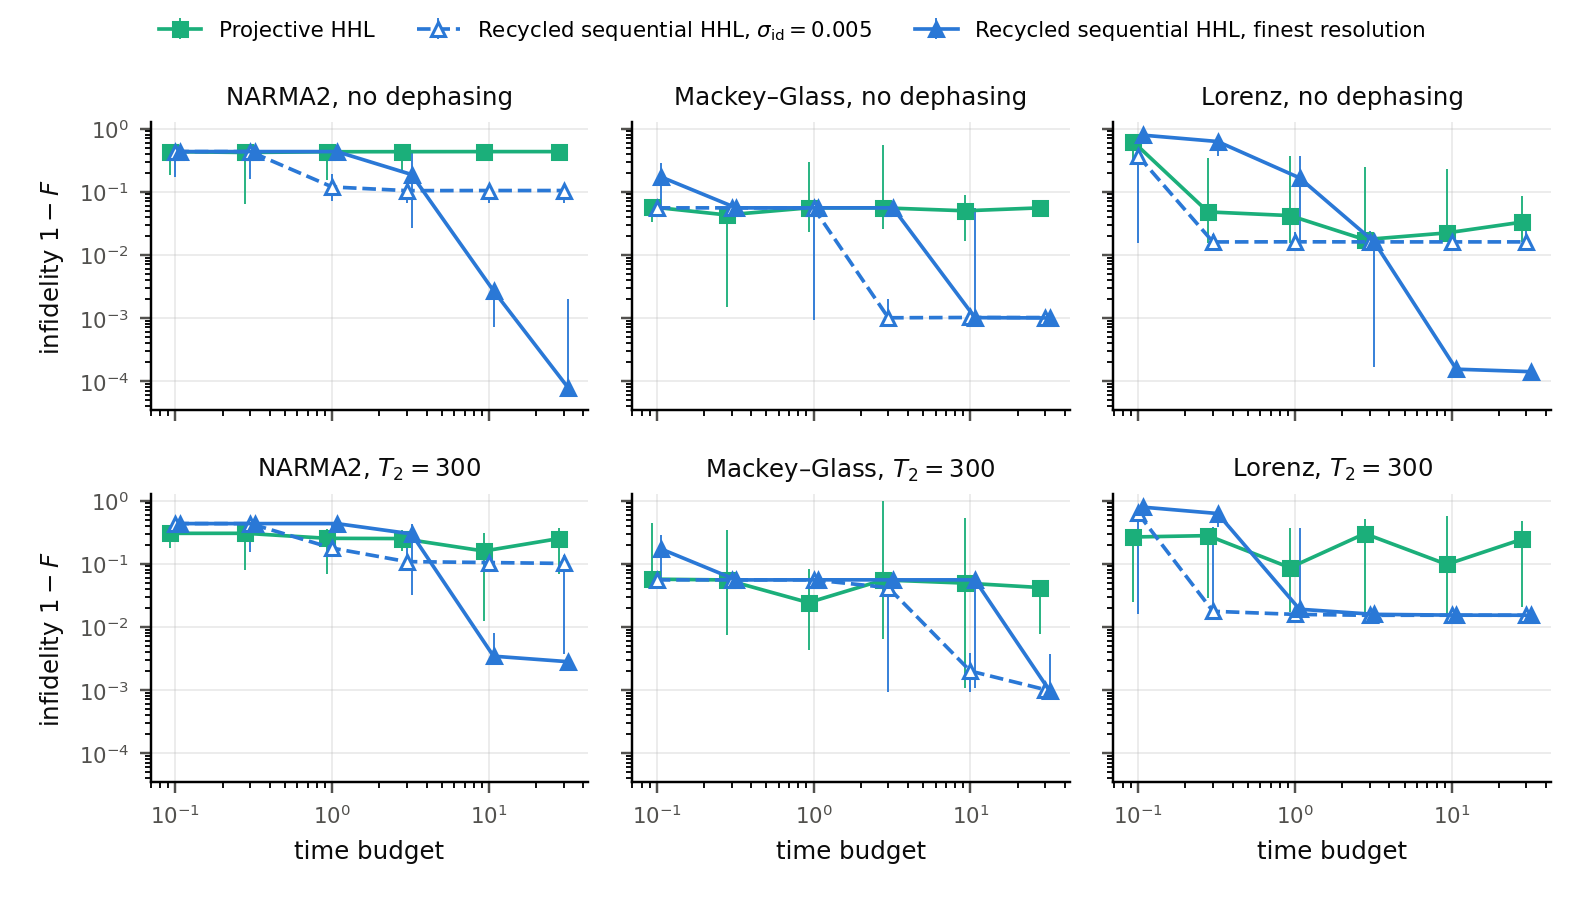
\includegraphics[width=0.92\textwidth]{figs/fig3_budget.png}
\caption{Median solution infidelity against the time budget on the three ridge systems of Table~\ref{tab:series}, without dephasing (top) and with $T_2=300$ (bottom). The unit of the budget is the median time of $10^4$ projective shots without dephasing; ten runs per point, bars from the lowest to the highest run, markers offset horizontally for visibility. Projective HHL (squares) has $10^4$ shots per unit and a six-bit register without dephasing, where its runs take between $0.79$ and $1.04$ of the budget, and at $T_2=300$ a five-bit register and the largest number of shots that keeps every run within the budget. The sequential estimator is run at $\sigma_{\rm id}=0.005$ (open triangles) and at the finest resolution used, $3\times10^{-4}$ without dephasing and $0.002$ at $T_2=300$ (filled triangles).}
\label{fig:budget}
\end{figure*}

\emph{Error against budget.} Fig.~\ref{fig:budget} shows Projective HHL and the sequential estimator at budgets from a tenth to thirty times the unit, the median time of $10^4$ projective shots without dephasing; the budget of Table~\ref{tab:series} is ten units, and every point has ten runs. The sequential estimator improves in steps, one for each group of weak components that its resolution separates. On NARMA2 without dephasing the median infidelity at the finest resolution is $0.43$ up to one unit, $0.19$ at three, $2.7\times10^{-3}$ at ten and $7.7\times10^{-5}$ at thirty. At $\sigma_{\rm id}=0.005$ the steps come earlier and end higher: on the Lorenz series without dephasing this resolution reaches $0.016$ at $0.3$ units and stays there, and the finest one reaches $0.016$ at three units and $1.5\times10^{-4}$ at ten. With $T_2=300$ both resolutions stay between $0.015$ and $0.019$ on this series from one unit to thirty. Projective HHL does not improve with the number of shots. On NARMA2 without dephasing its median infidelity is $0.42$ to $0.43$ from $10^3$ to $3\times10^5$ shots, and in the six settings its median at thirty units is between $0.8$ and $2.8$ times that at one unit.

\emph{At one unit.} At one unit, the budget of the tests of Secs.~\ref{sec:bench} to \ref{sec:grid}, the sequential estimator is not ahead throughout. Projective HHL has the lower median infidelity than the finest resolution in four of the six settings, one of them by less than $1\%$, and than $\sigma_{\rm id}=0.005$ in one: on the Mackey--Glass series at $T_2=300$ it reaches $0.024$ against $0.055$ for both resolutions, although it reproduces the ridge forecast in six runs there and the sequential estimator in all ten.

\emph{Forecast against budget.} The forecast follows only the first steps. From one unit on, the median NMSE of the three stages is within $0.07$ of that of the ridge readout in every setting, and within $0.12$ at a tenth of a unit; on NARMA2 without dephasing it is $0.15$ at one unit and $0.12$ at thirty for the finest resolution, while the infidelity falls from $0.43$ to $7.7\times10^{-5}$. At $\sigma_{\rm id}=0.005$ the sequential estimator reproduces the ridge forecast in all ten runs at every budget on the Mackey--Glass series, from $0.3$ units on the Lorenz series without dephasing and from one unit at $T_2=300$; on NARMA2 only the finest resolution does, from ten units. Projective HHL does so in all ten runs at two of its $36$ points. A larger budget is not always better at a fixed resolution: on NARMA2 at $T_2=300$ and $\sigma_{\rm id}=0.005$ the median $D$ is $0.063$ at one unit, against $0.005$ at a tenth of a unit.

\section{Baselines without phase estimation}
\label{sec:vqls}

\begin{table}[t]
\caption{Variational quantum linear solver on the systems of Tables~\ref{tab:learn}, \ref{tab:grid} and \ref{tab:series} and on the 118-bus system (last three rows: the ridge systems of the three series): median solution infidelity $1-F$ over ten runs from random angles, $n$ qubits. ``Terms'': Pauli terms measured for one value of the cost. ``Exact'': exact cost and gradient; ``pairs'': pairs of a circuit and a term evaluated by that run (median). Last two columns: stochastic optimisation within $10^4$ and $10^7$ circuit executions. ``--'': one iteration does not fit. Sub- and superscripts: lower and upper quartile of the runs, omitted where both equal the median as printed. No dephasing is applied (see the text).}
\label{tab:vqls}
\centering\footnotesize\renewcommand{\arraystretch}{1.3}
\setlength{\tabcolsep}{3pt}
\begin{tabular}{lcccccc}
\toprule
System & $n$ & terms & exact & pairs & $10^4$ & $10^7$\\
\midrule
Random $4\times4$ & 2 & 47 & $<$1e-9 & 1.3e4 & 0.690$_{0.616}^{0.798}$ & 0.023$_{0.015}^{0.032}$\\
Poisson $N=4$ & 2 & 9 & $<$1e-9 & 1.9e3 & 0.812$_{0.524}^{0.964}$ & 0.121$_{0.042}^{0.249}$\\
Poisson $N=8$ & 3 & 21 & $<$1e-9 & 1.6e4 & 0.839$_{0.698}^{0.972}$ & 0.865$_{0.799}^{0.920}$\\
Toeplitz $N=8$ & 3 & 33 & $<$1e-9 & 1.3e4 & 0.893$_{0.864}^{0.965}$ & 0.064$_{0.027}^{0.105}$\\
9-bus & 3 & 63 & $<$1e-9 & 7.2e4 & 0.946$_{0.919}^{0.962}$ & 0.447$_{0.260}^{0.667}$\\
14-bus & 4 & 223 & $<$1e-9 & 2.6e6 & 0.958$_{0.849}^{0.996}$ & 0.975$_{0.932}^{0.990}$\\
30-bus & 5 & 807 & $<$1e-9 & 1.2e8 & 0.963$_{0.904}^{0.994}$ & 0.966$_{0.950}^{0.999}$\\
118-bus & 7 & 8127 & 0.579$_{0.376}^{0.768}$ & 4.8e9 & -- & 0.994$_{0.990}^{0.997}$\\
NARMA2 & 4 & 256 & $<$1e-9 & 3.4e6 & 0.959$_{0.940}^{0.992}$ & 0.936$_{0.858}^{0.988}$\\
Mackey--Glass & 4 & 256 & $<$1e-9 & 2.0e6 & 0.959$_{0.889}^{0.991}$ & 0.967$_{0.944}^{0.986}$\\
Lorenz & 4 & 256 & $<$1e-9 & 1.2e6 & 0.971$_{0.942}^{0.990}$ & 0.952$_{0.929}^{0.975}$\\
\bottomrule
\end{tabular}
\end{table}

\begin{table}[t]
\caption{Forecast NMSE of baselines without phase estimation on the three series of Sec.~\ref{sec:series} (median of ten runs; one value where nothing is random). ``Ridge readout'': the exact readout of the echo state network. ``Exact'': exact expectation values, or exact cost for the variational solver; otherwise the number of circuit executions. DQI: the polynomial that satisfies most constraints among $10^5$ samples, for constraint sets of $r$ levels. Sub- and superscripts: lower and upper quartile of the runs, omitted where both equal the median as printed.}
\label{tab:nisq}
\centering\footnotesize\renewcommand{\arraystretch}{1.3}
\setlength{\tabcolsep}{4pt}
\begin{tabular}{lccc}
\toprule
Method & NARMA2 & Mackey--Glass & Lorenz\\
\midrule
Ridge readout, exact & 0.120 & 0.235 & 0.132\\
Last known value & 0.838 & 0.668 & 0.263\\
\midrule
Variational solver, exact & 0.120 & 0.235 & 0.132\\
Variational solver, $10^5$ & 0.968$_{0.791}^{1.028}$ & 0.691$_{0.635}^{0.770}$ & 0.437$_{0.282}^{0.791}$\\
Variational solver, $10^7$ & 0.396$_{0.268}^{0.667}$ & 0.567$_{0.395}^{0.769}$ & 0.348$_{0.275}^{0.476}$\\
Quantum reservoir, exact & 0.207 & 0.233 & 0.241\\
Quantum reservoir, $10^5$ & 0.642$_{0.624}^{0.660}$ & 0.560$_{0.548}^{0.577}$ & 0.433$_{0.428}^{0.442}$\\
Circuit learning, exact & 0.144$_{0.137}^{0.160}$ & 0.097$_{0.094}^{0.100}$ & 8.4e-3$_{7.5e-3}^{8.6e-3}$\\
Circuit learning, $10^5$ & 0.912$_{0.870}^{0.956}$ & 0.797$_{0.731}^{0.896}$ & 0.623$_{0.478}^{1.047}$\\
DQI, $r=5$, $10^5$ & 1.204 & 1.639 & 0.837\\
DQI, $r=15$, $10^5$ & 1.609$_{1.365}^{1.609}$ & 0.655$_{0.655}^{0.971}$ & 0.267$_{0.259}^{0.267}$\\
\bottomrule
\end{tabular}
\end{table}

Variational solvers prepare the solution without phase estimation and are the usual proposal for devices without error correction. We run the variational quantum linear solver \cite{BravoPrieto2023} on the four systems of Table~\ref{tab:learn}, on the 9-, 14-, 30- and 118-bus systems of Sec.~\ref{sec:grid} and on the three ridge systems of Sec.~\ref{sec:series}, with the dimension padded to a power of two by a unit block. The trial state $|\psi\rangle$ of $n$ qubits is prepared by layers of single-qubit rotations $R_Y$ ($R_Y$ and $R_Z$ on the complex system) separated by a chain of CNOT gates, with one layer more than the number of free amplitudes requires, and the angles minimise the global cost $C=1-|\langle b|A|\psi\rangle|^2/\langle\psi|A^2|\psi\rangle$.

\emph{Cost unit and protocols.} The unit of cost of this solver is a circuit execution, not evolution time, and none of its circuits contains the controlled evolution to which $T_2$ refers; only the calibrated read-out contrast $1-p_d$ is applied. We therefore compare by the number of state preparations, which is $10^4$ for the learning stages of Tables~\ref{tab:learn} and \ref{tab:grid}. Two protocols are run, ten times each from random angles. In the first the cost and its gradient are exact and the optimiser is L-BFGS with at most $4000$ iterations; this is the ceiling of the method, and we count the pairs of a circuit and a Pauli term that it evaluates, which is the number of executions at one shot per pair. In the second the cost is estimated within a fixed number of executions, $\langle b|A|\psi\rangle$ from one Hadamard test per Pauli term of $A$ and $\langle\psi|A^2|\psi\rangle$ from the Pauli terms of $A^2$, and the angles follow simultaneous-perturbation stochastic approximation \cite{Spall1992}; every term gets the largest number of shots that leaves $500$ iterations, and at least one. The fidelity of the final state is computed exactly in both protocols.

\emph{Results.} With an exact cost the median infidelity is below $10^{-9}$ on ten systems (Table~\ref{tab:vqls}): every run is below $10^{-9}$ on the nine smaller ones, and on the 30-bus system nine runs are below $10^{-8}$ and one, which stops at the iteration limit, ends at $1.6\times10^{-4}$. On the 118-bus system all ten runs stop at the iteration limit, with a median of $0.58$. The exact runs on the ten systems evaluate between $1.9\times10^3$ and $1.2\times10^8$ pairs (medians), more than the $10^4$ state preparations of the learning stages on all of them except Poisson $N=4$. Within $10^4$ executions the median infidelity is between $0.69$ and $0.97$, as for a random state (expected $1-2^{-n}$, $0.75$ to $0.97$), with single runs between $0.18$ and $1.00$; on the 118-bus system, whose cost has $8127$ terms, one iteration does not fit. Within $10^7$ executions the median falls to $0.023$--$0.45$ on the random, the Poisson $N=4$, the Toeplitz and the 9-bus system and stays above $0.8$ on the other seven.

\emph{Cost and fidelity.} On Poisson $N=8$ the runs within $10^7$ executions end at a median cost of $0.052$ and a median infidelity of $0.865$. The cost bounds the infidelity only as $C\ge(1-F)/\kappa^2$ \cite{BravoPrieto2023}, so a small cost does not certify a state near the solution when $\kappa$ is large. The entries of Table~\ref{tab:vqls} are for one plain implementation: a global cost, no grouping of commuting terms, step sizes of the stochastic optimiser fixed after a small trial on the Poisson $N=4$ system, and ten repetitions. They are not a bound for variational solvers, and the number of pairs depends on the path of the optimiser. The comparison is also between resources of different kinds: a state preparation of a learning stage is followed by controlled evolution of up to $t_{\rm cap}$, which the variational circuits do not contain.

\emph{Forecasting models.} For the series of Sec.~\ref{sec:series} we add three methods that produce forecasts without solving the ridge system by phase estimation (Table~\ref{tab:nisq}). The first is a quantum reservoir of four qubits \cite{Fujii2017}: at every step the first qubit is reset to $\sqrt{1-s}|0\rangle+\sqrt s|1\rangle$ with the input $s$ scaled to $[0,1]$, the register evolves for unit time under $H=\sum_{i<j}J_{ij}X_iX_j+\sum_iZ_i$ with $J_{ij}$ uniform in $[-1,1]$, and $\langle Z_i\rangle$ is read at four equally spaced times, which gives sixteen features for the ridge readout of Sec.~\ref{sec:series}. Each measured step and time is one circuit, $12\,000$ in all. The second is quantum circuit learning \cite{Mitarai2018} with four qubits: three layers each encode the last four inputs by $R_Y(\arcsin x)R_Z(\arccos x^2)$ and apply a CNOT chain and trainable rotations $R_YR_Z$; the forecast is $a\langle Z_1\rangle+c$, and the $26$ parameters minimise the squared error on the training steps, by L-BFGS with exact expectation values ($300$ iterations) or by stochastic approximation on minibatches of $100$ samples with two independent shots each; the two one-shot residuals of a sample are multiplied, which estimates its squared error without bias.

\emph{Decoded quantum interferometry.} The third method, decoded quantum interferometry (DQI) \cite{Jordan2025}, is an optimisation algorithm and not a linear solver. We apply it to optimal polynomial intersection, the problem on which it is analysed: a polynomial of degree at most four over $\mathbb F_{31}$ maps the level of the most recent input on which the target depends ($30$ levels) to the level of the target ($31$ levels), and the constraint set of an input level holds the $r$ output levels around the median training target of that level, with $r=5$ and $r=15$. The code dual to the instance is a Reed--Solomon code of distance six, so the DQI polynomial has degree two. We sample from the exact output distribution of the ideal algorithm with perfect decoding, obtained by enumerating all $31^5$ polynomials; its norm and its expected number of satisfied constraints agree with Lemmas~9.1 and 9.2 of \cite{Jordan2025} to $10^{-9}$ and $10^{-6}$.

\emph{Forecasts.} With exact expectation values the quantum reservoir gives NMSE $0.21$, $0.23$ and $0.24$, and the trained circuit $0.14$, $0.097$ and $0.0084$. The circuit is better than the regularised ridge readout on the Mackey--Glass and Lorenz series; it is not bound by $\kappa\le100$, and its exact training evaluates $9\times10^6$ to $3\times10^7$ circuits. Within $10^5$ executions, the number of state preparations of Projective HHL in Table~\ref{tab:series} without dephasing, the reservoir has eight shots per circuit and gives $0.64$, $0.56$ and $0.43$, the trained circuit gives $0.91$, $0.80$ and $0.62$, and the readout of the variational solver gives $0.97$, $0.69$ and $0.44$. With $10^4$ executions the circuits of the reservoir cannot each be run once.

One DQI sample satisfies $30\%$ ($r=5$) and $64\%$ ($r=15$) of the constraints, against $16\%$ and $48\%$ for a random polynomial, and the best of $10^5$ samples satisfies in the median as many as the optimum found by exhaustive search, $63\%$ and $97\%$ to $100\%$. The forecasts of these polynomials have NMSE between $0.66$ and $1.6$, and $0.27$ on the Lorenz series with $r=15$, the level of repeating the last known value. The limit is not the sampling: the best sample already reaches the optimum of the objective, and that objective counts satisfied constraints and does not measure the squared error of a forecast. In this formulation a level whose constraint is not met receives a value unrelated to the target.

\emph{Number of executions.} Between $10^4$ and $10^7$ executions (seven values, ten runs each) the forecast of the quantum reservoir improves steadily, from NMSE $0.86$, $0.79$ and $0.60$ at $3\times10^4$ executions to $0.24$, $0.24$ and $0.25$ at $10^7$, close to its values with exact expectation values. The trained circuit improves unevenly, from $1.00$, $0.87$ and $1.04$ at $10^4$ executions to $0.59$, $0.59$ and $0.41$ at $10^7$. The readout of the variational solver shows no trend, with a median infidelity above $0.9$ at every number of executions, and the forecasts of the best DQI sample stay between $0.26$ and $1.9$ from $10^5$ samples on.

\emph{Scope of these baselines.} The forecasting models differ from the linear solvers in the task they are given, in their input and in their unit of cost, so Table~\ref{tab:nisq} gives reference levels and not a ranking. The reservoir couplings, the depth of the trained circuit, the field size and the degree were fixed beforehand and not tuned, each method is one plain implementation with ten runs, and no dephasing is applied to them. With exact expectation values the variational solver reproduces the ridge readout and the trained circuit is better than it on two series, at $10^6$ to $3\times10^7$ evaluations of a circuit or of a circuit and a term. Within $10^5$ executions none of the four methods comes near the ridge readout, and only the quantum reservoir on NARMA2 and Mackey--Glass and DQI with $r=15$ on Mackey--Glass are below the error of repeating the last known value.

\section{A system register of finite lifetime}
\label{sec:system}

\begin{table*}[t]
\caption{Recycled sequential HHL when a copy loses its eigencomponent at a rate $1/T_{\rm sys}$ and continues in a component drawn with the weights of the input (redrawing) or uniformly from all eigenvectors (depolarising); no dephasing, ten runs, median with the quartiles as sub- and superscripts. Poisson $N=8$: $T_{\rm tot}=2\times10^6$; 9-bus: the protocol of Table~\ref{tab:grid}; Lorenz readout: that of Table~\ref{tab:series} at the finest resolution. Without system noise the longest copy of a run lasts $3.3\times10^4$, $3.4\times10^4$ and $1.2\times10^5$ time units on the three systems in the median of the runs, and at most $1.4\times10^5$ on the Lorenz readout ($2.3\times10^5$ with system noise). The infidelity does not use the learned weights; the compliance does.}
\label{tab:system}
\centering\footnotesize\renewcommand{\arraystretch}{1.3}
\setlength{\tabcolsep}{3pt}
\begin{tabular}{lccccccc}
\toprule
$T_{\rm sys}$ & $\infty$ & $3\times10^6$ & $10^6$ & $3\times10^5$ & $10^5$ & $3\times10^4$ & $10^4$\\
\midrule
\multicolumn{8}{l}{\emph{Solution infidelity $1-F$}}\\
Poisson $N=8$, redrawing & 2.5e-6$_{2.4e-6}^{2.6e-6}$ & 2.5e-6$_{2.4e-6}^{2.6e-6}$ & 2.5e-6$_{2.4e-6}^{2.6e-6}$ & 2.5e-6$_{2.4e-6}^{2.6e-6}$ & 2.4e-6$_{2.4e-6}^{2.8e-6}$ & 5.0e-6$_{3.7e-6}^{9.2e-6}$ & 3.1e-5$_{1.5e-5}^{5.4e-5}$\\
Poisson $N=8$, depolarising & 2.5e-6$_{2.4e-6}^{2.6e-6}$ & 2.5e-6$_{2.4e-6}^{2.6e-6}$ & 2.5e-6$_{2.4e-6}^{2.6e-6}$ & 2.4e-6$_{2.4e-6}^{2.7e-6}$ & 2.5e-6 & 9.7e-7$_{1.6e-7}^{2.2e-6}$ & 5.7e-6$_{1.4e-6}^{1.5e-5}$\\
9-bus, redrawing & 4.3e-7$_{2.3e-7}^{8.6e-7}$ & 5.0e-7$_{2.7e-7}^{9.6e-7}$ & 6.1e-7$_{5.7e-7}^{1.1e-6}$ & 6.5e-7$_{2.5e-7}^{1.4e-6}$ & 2.6e-6$_{1.4e-6}^{4.7e-6}$ & 2.1e-5$_{1.3e-5}^{2.5e-5}$ & 8.4e-5$_{7.4e-5}^{9.7e-5}$\\
9-bus, depolarising & 4.3e-7$_{2.3e-7}^{8.6e-7}$ & 4.4e-7$_{3.0e-7}^{5.0e-7}$ & 4.4e-7$_{2.8e-7}^{6.2e-7}$ & 1.8e-7$_{1.5e-7}^{9.7e-7}$ & 1.2e-6$_{2.9e-7}^{1.5e-6}$ & 2.3e-6$_{7.2e-7}^{5.6e-6}$ & 1.3e-5$_{5.7e-6}^{3.9e-5}$\\
Lorenz readout, redrawing & 1.5e-4$_{1.4e-4}^{1.6e-4}$ & 1.5e-4$_{1.4e-4}^{1.6e-4}$ & 1.6e-4$_{1.4e-4}^{1.7e-4}$ & 1.5e-4$_{1.4e-4}^{1.5e-4}$ & 1.8e-4$_{1.7e-4}^{2.7e-4}$ & 0.017$_{6.2e-4}^{0.017}$ & 0.017$_{0.017}^{0.268}$\\
Lorenz readout, depolarising & 1.5e-4$_{1.4e-4}^{1.6e-4}$ & 1.4e-3$_{2.1e-4}^{1.5e-3}$ & 1.7e-4$_{1.4e-4}^{1.9e-4}$ & 1.5e-4$_{1.4e-4}^{1.8e-4}$ & 1.6e-4$_{1.5e-4}^{1.9e-4}$ & 4.2e-4$_{3.2e-4}^{5.0e-4}$ & 1.8e-3$_{1.4e-3}^{2.0e-3}$\\
\midrule
\multicolumn{8}{l}{\emph{Error of the compliance (\%)}}\\
Poisson $N=8$, redrawing & 2.5$_{2.0}^{4.1}$ & 4.4$_{2.6}^{5.5}$ & 3.3$_{1.7}^{5.1}$ & 2.6$_{1.7}^{3.0}$ & 2.5$_{1.2}^{4.2}$ & 1.3$_{0.50}^{3.4}$ & 4.3$_{3.5}^{5.9}$\\
Poisson $N=8$, depolarising & 2.5$_{2.0}^{4.1}$ & 4.4$_{1.1}^{6.1}$ & 1.6$_{0.80}^{5.9}$ & 2.6$_{2.0}^{3.8}$ & 3.1$_{2.0}^{4.5}$ & 4.5$_{2.0}^{6.3}$ & 5.6$_{3.9}^{7.7}$\\
9-bus, redrawing & 0.19$_{0.12}^{0.29}$ & 0.27$_{0.09}^{0.43}$ & 0.16$_{0.09}^{0.25}$ & 0.14$_{0.04}^{0.19}$ & 0.38$_{0.28}^{0.64}$ & 0.33$_{0.29}^{0.49}$ & 0.39$_{0.16}^{0.65}$\\
9-bus, depolarising & 0.19$_{0.12}^{0.29}$ & 0.14$_{0.09}^{0.36}$ & 0.30$_{0.10}^{0.51}$ & 0.25$_{0.15}^{0.58}$ & 0.80$_{0.43}^{1.1}$ & 3.3$_{3.1}^{3.7}$ & 8.9$_{8.4}^{9.5}$\\
Lorenz readout, redrawing & 0.50$_{0.31}^{0.72}$ & 0.72$_{0.31}^{1.0}$ & 0.66$_{0.28}^{0.78}$ & 0.61$_{0.36}^{1.0}$ & 1.7$_{0.96}^{2.3}$ & 4.8$_{4.3}^{5.1}$ & 8.3$_{7.9}^{8.6}$\\
Lorenz readout, depolarising & 0.50$_{0.31}^{0.72}$ & 5.6$_{4.6}^{6.6}$ & 18$_{18}^{19}$ & 62$_{60}^{64}$ & 185$_{180}^{193}$ & 648$_{638}^{662}$ & 2099$_{2037}^{2170}$\\
\bottomrule
\end{tabular}
\end{table*}

Equation~\eqref{eq:record} holds while the system register is disturbed only by the measurements. Table~\ref{tab:system} extends the test of Sec.~\ref{sec:bench} to two models and three systems. In both models a copy loses its eigencomponent at a rate $1/T_{\rm sys}$, during identification and during refinement, and continues in a component drawn afresh: with the weights $w_j$, as if the register were prepared again in $|b\rangle$ (redrawing), or uniformly from all $N$ eigenvectors, a reset of the populations that stands for a depolarised register and is called depolarising below. A jump is applied at the start of a measurement, whose whole evolution then runs with the new eigenvalue; a transition during a controlled evolution and coherences between eigenspaces are not modelled.

\emph{Protocol and metric.} The systems are Poisson $N=8$, the 9-bus system of Sec.~\ref{sec:grid} and the Lorenz readout of Sec.~\ref{sec:series} at its finest resolution, without dephasing and with $\delta=10^{-3}$; the runs with $T_{\rm sys}=\infty$ are those of Tables~\ref{tab:grid} and \ref{tab:series}. Without system noise a copy takes $23$, $20$ and $21$ identification measurements on the three systems (the copies cut off at the end of the budget are counted) and lasts $7.2\times10^2$, $7.1\times10^2$ and $3.3\times10^3$ time units on average; refinement adds $5\times10^2$ to $1\times10^3$ measurements to a whole run. The infidelity is that of the idealised solver, which applies the inverse of the learned value nearest to each eigencomponent and does not use the learned weights. It can therefore fall when jumps add learned values, and it does not show damage to the weights; the compliance, which uses them, does.

\emph{Eigenvalues, redrawing.} The median infidelity stays within a factor $1.6$ of its value without system noise for $T_{\rm sys}\ge3\times10^5$. Below that it rises: on Poisson $N=8$ to $5.0\times10^{-6}$ at $T_{\rm sys}=3\times10^4$ and $3.1\times10^{-5}$ at $10^4$, on the 9-bus system to $8.4\times10^{-5}$ at $10^4$, with a worst run of $2.6\times10^{-4}$ against $0.19$ to $0.23$ for the other learning stages of Table~\ref{tab:grid}, and on the Lorenz readout to $0.017$ at $3\times10^4$, where only four components are learned in six of ten runs, against five without system noise; the worst run on that system is $0.37$, at $10^4$. The Lorenz copies are the longest, and the lifetime at which the estimator fails on that system is a quarter of its longest copy and nine times its mean copy. For $T_{\rm sys}\ge10^5$ no learned value lies farther than $4\sigma_{\rm id}$ from an eigenvalue.

\emph{Eigenvalues, depolarising.} The median infidelity is at most $1.4\times10^{-5}$ on Poisson $N=8$ and on the 9-bus system at every lifetime, with worst runs of $0.013$ and $8.1\times10^{-3}$ at $T_{\rm sys}=10^4$ and one of $5.1\times10^{-3}$ at $10^5$ on the 9-bus system. On the Lorenz readout it is $1.5\times10^{-4}$ to $1.7\times10^{-4}$ for $10^5\le T_{\rm sys}\le10^6$, $4.2\times10^{-4}$ at $3\times10^4$ and $1.8\times10^{-3}$ at $10^4$. At the two shortest lifetimes the medians are lower than with redrawing on all three systems, which is consistent with uniform jumps carrying copies to the weak components: on Poisson $N=8$ eight values are learned in seven of ten runs at $T_{\rm sys}=3\times10^4$ and in all ten at $10^4$, against seven values in eight of ten runs without system noise, and the metric does not use the weights.

\emph{A merged cluster.} On the Lorenz readout the median at $T_{\rm sys}=3\times10^6$ is higher than at shorter lifetimes, $1.4\times10^{-3}$: six of ten runs lie between $1.4\times10^{-3}$ and $1.7\times10^{-3}$ and four between $2.4\times10^{-5}$ and $2.5\times10^{-4}$. The learned values show the cause. Without system noise the lowest learned value is $0.0110$ to $0.0113$ in every run and carries five to thirteen copies; it stands for the two weak components next above the regularisation floor at $0.0100$. In the six runs it is $0.0101$ to $0.0102$ with $41$ to $68$ copies: the copies that jumped to the floor outnumber those of the weak components, are clustered with them and set the learned value. With more jumps the floor is learned as a value of its own, in eight of ten runs at $T_{\rm sys}=10^6$ and in nine at $3\times10^5$.

\emph{Weights.} Depolarisation damages the weights at lifetimes that leave the eigenvalues intact. A copy that jumps is labelled with an eigenvalue drawn uniformly, so a share of the copies of the order of the mean copy time over $T_{\rm sys}$, divided among the $N$ eigenvectors, is added to every weight. On the Lorenz readout ten of the sixteen eigenvalues lie at the regularisation floor and hold $1.0\times10^{-7}$ of the weight. The compliance, which weighs each component by $1/\lambda_j$, is in error by $0.5\%$ without system noise, by $5.6\%$ at $T_{\rm sys}=3\times10^6$, where about one copy in a thousand jumps, by $62\%$ at $3\times10^5$ and by more than $100\%$ from $10^5$ on; with redrawing the error is at most $1.7\%$ down to $10^5$ and $8.3\%$ at $10^4$. From $T_{\rm sys}=10^5$ on, values far from every eigenvalue are learned as well, in the median $1$, $4$ and $11$ per run at $10^5$, $3\times10^4$ and $10^4$. On the 9-bus system the compliance error is below $1\%$ for $T_{\rm sys}\ge10^5$ and $3.3\%$ and $8.9\%$ at $3\times10^4$ and $10^4$ ($0.4\%$ at most with redrawing); on Poisson $N=8$ it is between $1.3\%$ and $5.6\%$ in every setting, $2.5\%$ without system noise.

\emph{Reading.} With redrawing, the median infidelity of the idealised solver is within a factor $1.6$ of its value without system noise down to $T_{\rm sys}=3\times10^5$, two and a half times the longest Lorenz copy and nine times the longest copy of the other two systems, and the estimator fails on the Lorenz readout at a quarter of its longest copy. With depolarising that infidelity stays at or below $1.4\times10^{-5}$ on the two smaller systems and below $2\times10^{-3}$ on the Lorenz readout at every lifetime, but it does not see the weights. The weights, and the observables of Sec.~\ref{sec:solver} computed from them, need the weight added by the jumps to be small against the weights of interest, a far stronger condition when the register depolarises; subtracting a known jump process was not attempted. Both are models of population transfer at the measurement boundaries and not gate-level simulations, the ancilla has no dephasing in these runs, and Projective HHL, whose shots last about $2\times10^3$ time units, was not run under them, so the results do not establish a tolerance to hardware noise.

\section{Discussion}
\label{sec:disc}

Five conclusions follow, each for the systems, the noise model and the time budgets studied; the first two rest on the four small systems, and Secs.~\ref{sec:grid} to \ref{sec:system} mark their limits.

First, for a non-eigenstate input the quantity that decides the learning stage is the detection of weak components. Mixture estimators need $S\gtrsim w_j^{-2}$ shots, a clock register needs $S\gtrsim w_j^{-1}$ down to a floor of a few per cent, and because a component that is missed at a small eigenvalue, or merged with one, dominates the error of the solution, this decides the fidelity; the counting model of \eqref{eq:count} summarises the two labelled cases and is an analogy for the mixture case.

Second, the floor is not intrinsic to labelling. Keeping the copy and labelling it by its own posterior, as Recycled sequential HHL does, replaces the register tail by a stopping threshold, removes the register and the QFT from the learning stage, frees the resolution from a register size and the detection from knowledge of the number of components. Within the same time budget, the median time of the register-labelled runs, the median solution infidelity is then lower than with register labels on every system and noise setting, by factors from $2$ to $3\times10^3$ when both estimators refine on every sample and from $1.5$ to $2\times10^3$ when both stop at a precision target. The advantage persists under both allocation policies; the comparison is between whole estimators and does not isolate the label. The price is a system register that must outlive a whole copy (Sec.~\ref{sec:system}: in two jump models the infidelity of the idealised solver is unchanged down to a few times the longest copy, while a depolarised register corrupts the learned weights at a lifetime more than twenty times that copy), a label error that is tuned through the stopping threshold and measured, not bounded (a matched noise model is necessary for the working model and not sufficient), and a sample that costs two to sixteen register labels.

Third, for a sparse spectral measure the learned atoms answer $\langle b|f(A)|b\rangle$ questions, and through polarisation linear functionals, by classical post-processing, as far as the learned weights are accurate; the weights are the first casualty of a depolarised system register (Sec.~\ref{sec:system}). Neither labelled estimator is uniformly better for the compliance and the energy, and more register shots do not systematically lower the projective error; at the larger observable budget the sequential estimator is the more accurate for linear functionals in all eight settings of the four small systems, most clearly where eigenvalues share a register bin; on the 30-bus power-flow system the projective estimator is the more accurate for the line flow in four of five settings.

Fourth, the learned spectrum does not by itself repair a hybrid solver for the remaining observables: with a uniform clock the loss is dominated by leakage, which a tapered clock removes when the register resolves the spectrum and there is no dephasing, and the spectrum is otherwise most valuable for choosing $t_0$ or, when it is fully captured and its nodes are accurate enough, for spectrally corrected inversion.

Fifth, under dephasing the coherent clock limits the solver for every estimator and clock state tested, while the learning stage needs no coherent register; its own requirement is the lifetime of the system register: a few times the longest copy for the eigenvalues in the jump models tested, and far longer for the weights if the register depolarises.

The power-flow test of Sec.~\ref{sec:grid} is consistent with the first two conclusions on spectra that were not constructed for the purpose and marks their limit: a component with $0.2\%$ of the weight at the smallest eigenvalue limits the fidelity of the 9-bus solution and, without dephasing, is assigned a learned value in all ten runs of Recycled sequential HHL, in at most $31$ of 100 runs of a mixture estimator and in no run of the QPE histograms and of Projective HHL, whereas with dephasing, or with twenty weighted components at the budget of Table~\ref{tab:grid}, no learning stage resolves the spectrum.

The forecasting test of Sec.~\ref{sec:series} adds a problem in which the weak components are weaker still. Within ten times the budget of the other tests Recycled sequential HHL at its finest resolution reproduces the forecast of the exact ridge readout in all ten runs on the three series, with and without dephasing; Projective HHL does so in none to nine runs and gains nothing from ten times the shots on NARMA2; at the budget of the other tests it has the lower median infidelity in some settings. The forecast error is far less sensitive than the fidelity, the resolution was compared after the runs, and the baselines without phase estimation of Sec.~\ref{sec:vqls} reach the ridge readout only with exact expectation values.

\begin{table*}[t]
\caption{Learning stages for a hybrid solver. ``Condition stated in the cited work'': what its analysis assumes about the input and the spectrum, a sufficient condition of its precision guarantee and not a condition of the counting model; the first three mixture rows are run here as plain implementations in the spirit of the cited methods and are given the dimension as the number of components. ``Samples to find a weight $w$'': the laws of Sec.~\ref{sec:setting}, which follow from the statistics of a sample and are not results of the cited works; $z$ is the detection threshold and $w_{\rm fl}$ the weight leaking into the label. $n_c$ from \eqref{eq:nc}.}
\label{tab:position}
\centering\footnotesize\renewcommand{\arraystretch}{1.25}
\setlength{\tabcolsep}{3pt}
\begin{tabular}{>{\raggedright\arraybackslash}p{3.3cm}>{\raggedright\arraybackslash}p{1.8cm}>{\raggedright\arraybackslash}p{2.4cm}>{\raggedright\arraybackslash}p{4.2cm}>{\raggedright\arraybackslash}p{2.3cm}>{\raggedright\arraybackslash}p{2.4cm}}
\toprule
Learning stage & Ancillas & One sample is & Condition stated in the cited work & Samples to find a weight $w$ & Run here\\
\midrule
Time series, matrix pencil \cite{OBrien2019} & 1 & a mixture outcome \eqref{eq:p} & unbiased for a target weight well above $1/K$ with $K$ time steps (expected; numerical study) & $z^2/w^2$ & ``Bayesian clock'', Tables~\ref{tab:grid}, \ref{tab:series}\\
MM-QCELS \cite{DingLin2023} & 1 & a mixture outcome & number of dominant eigenvalues known; gap between them; each has more than three times the weight of the rest & $z^2/w^2$ & Tables~\ref{tab:learn}, \ref{tab:grid}, \ref{tab:series}\\
QMEGS \cite{QMEGS2024} & 1 & a mixture outcome & an upper bound on the number of dominant eigenvalues; the smallest dominant weight exceeds the total weight of the others; no gap needed & $z^2/w^2$ & Tables~\ref{tab:learn}, \ref{tab:grid}, \ref{tab:series}\\
QCELS \cite{QCELS2023} & 1 & a mixture outcome & one eigenvalue with weight above $0.71$, or a filtered input & -- & no (one eigenvalue)\\
Robust multiple-phase estimation \cite{RMPE2023} & 1 & a mixture outcome & number of dominant eigenvalues and bounds on their weights known & $z^2/w^2$ & no\\
Sampled QPE \cite{Lee2019,Yalovetzky2024,Morgan2025} & $n$; one if semiclassical \cite{Yalovetzky2024} & a register label & eigenvalues exact on the register \cite{Lee2019}; time scale learned \cite{Yalovetzky2024} & $z^2(w+w_{\rm fl})/w^2$, floor $w\gtrsim w_{\rm fl}$ & $n=6,8,10$, Tables~\ref{tab:learn}, \ref{tab:grid}, \ref{tab:series}\\
Iterative phase estimation as used in \cite{Gao2021} & 1 & the digits of one copy & eigenvalues are exact binary fractions & -- & no (not met by the test spectra)\\
\midrule
Projective HHL & $n_c+1$ & a register label, then a refinement outcome & smallest gap known (this work) & $z^2(w+w_{\rm fl})/w^2$, floor $w\gtrsim w_{\rm fl}$ & Secs.~\ref{sec:bench} to \ref{sec:series}\\
Recycled sequential HHL & 1 & the record of one kept copy \eqref{eq:record} & smallest gap known; system register outlives a copy (this work) & $z^2(w+w_{\rm fl})/w^2$, with $w_{\rm fl}$ set by $p_{\rm out}$: measured (Table~\ref{tab:cost}), not bounded & Secs.~\ref{sec:bench} to \ref{sec:series} and \ref{sec:system}\\
\bottomrule
\end{tabular}
\end{table*}

Several limitations should be stated.

\emph{Noise model.} The noise model is a calibrated contrast on the control qubit and a fixed depolarising rate; gate-level noise on the system register, independent noise in the inverse QPE and miscalibration of the coarse stage were not modelled. For the sequential estimator this matters more than for the others. Equation~\eqref{eq:record} holds only while the system register evolves under $A$ alone, so Trotter error and system noise that moves population between eigenspaces are outside it; a copy must survive for $9\times10^2$ to $8\times10^4$ time units on the four small systems, depending on the allocation and the resolution, and for up to $1.4\times10^5$ on the Lorenz readout without system noise; and the system-noise tests of Sec.~\ref{sec:system} are two models of population transfer without ancilla dephasing, not gate-level simulations.

\emph{Stopping threshold and resolution.} The stopping threshold is not an error bound: a matched contrast is necessary for the working model but not sufficient for coverage with the tempered likelihood and the plug-in prior, the measured error fractions are simulation results for one system, and with an over-estimated contrast they exceed the threshold by up to a factor of seventeen. The resolution is uniform, so that one close pair makes every copy expensive, and $\sigma_{\rm id}$, like $n_c$, is set from the smallest gap, which is assumed known.

\emph{Prior art.} The building blocks are known: the record identity of repeated ancilla measurements \cite{OBrien2019} and its back-action \cite{Jin2023}, Bayesian phase estimation of several eigenvalues with fitted weights \cite{vandenBerg2021}, iterative phase estimation inside a hybrid solver \cite{Gao2021}, rate-of-gain experiment design \cite{deNeeve2025,McMichael2021} and window states for the clock \cite{HHL2009,Rendon2022,Patel2026,Kristjuhan2026}. The two detection laws have precedents for single estimators and for uniform weights \cite{OBrien2019,QMEGS2024,Izumi2026}. Table~\ref{tab:position} sets the learning stages compared here next to the methods they follow, with the conditions those works state. The contribution is the combination of the building blocks into a learning stage, the reading of the laws as a design criterion for the learning stage, and the numerical study on small instances; a guarantee on the label error, optimality of the cost and a matched-time advantage beyond the tested settings are not established.

\emph{Statistics and baselines.} The comparisons between estimators use independent repetitions, not common random numbers, and the five to ten repetitions of the matched-time comparisons do not resolve rare failures: in Table~\ref{tab:matched} the projective result on Poisson $N=8$ at $T_2=300$ has two groups (seven of ten runs near $0.076$, three below $4\times10^{-4}$), ``worst'' means the worst of the runs made, and only Table~\ref{tab:learn}, with 100 repetitions, estimates the frequency of such failures; its reliability does not carry over to the other tables. The mixture baselines are plain implementations: the MM-QCELS-type estimator misses components that a tuned estimator would find (it fails at $w_j\sqrt S\approx10$ where the QMEGS-type estimator succeeds), so the measured gap between mixture and labelled estimators is an upper bound on the gap implied by the detection law.

\emph{Test set and repetitions.} The test set is four systems with $N\le8$, three power-flow systems and three ridge systems of one reservoir, with one input vector each, and the repetition counts (100 for Table~\ref{tab:learn}, three for Fig.~\ref{fig:T2}, ten for Tables~\ref{tab:matched}, \ref{tab:clock}, \ref{tab:window}, \ref{tab:series}, \ref{tab:vqls}, \ref{tab:nisq} and \ref{tab:system} and for Fig.~\ref{fig:budget}, five at the full Toeplitz resolution, six for Table~\ref{tab:qoiseq} and the spectral columns of Table~\ref{tab:qoi}, four for its Krylov and Fourier columns, forty learning runs for Table~\ref{tab:poly}; in Sec.~\ref{sec:grid} 100 for the mixture and QPE rows of Table~\ref{tab:grid}, ten for its two labelled estimators and five at the finest resolution, six for the observables, five for the scaling runs and four for the model-free estimators) are, except for Table~\ref{tab:learn} and the upper rows of Table~\ref{tab:grid}, small for outcomes with two groups; medians are reported with interquartile ranges where they are wide in Table~\ref{tab:learn} and with both quartiles in Tables~\ref{tab:grid}, \ref{tab:series}, \ref{tab:vqls}, \ref{tab:nisq} and \ref{tab:system} (linear interpolation between the ordered runs).

\emph{Idealisations.} The weight estimation of the projective estimator assumes the clock kernel is known, which requires the learned eigenvalues and the dephasing model; a kernel mismatch biases the weights directly. The clock analysis uses the ideal circuit with exact Hamiltonian simulation and does not include block-encoding subnormalisation or QSVT phase-factor synthesis, and the interval reference polynomial is a bounded linear-program solution rather than a Remez construction.

\emph{Scaling.} For generic inputs the number of learned components grows with the dimension, and the learning cost then removes any asymptotic advantage; the analysis is intended for structured problems with few weighted components, the regime in which hybrid solvers are proposed, and the Krylov baseline used here is the plain thresholded variant rather than the stabilised constructions of \cite{YuZhou2026,Park2026}. Instance-dependent complexities of this kind have been formalised for fully coherent solvers \cite{Dalzell2026}; the present work gives the corresponding statement for the learning stage and for the observables it already determines.

\appendices
\section{Proofs and algorithms}
\label{app:proofs}

\emph{Weight information.} For a Bernoulli outcome with probability $p$ the Fisher information on a parameter $\vartheta$ is $(\partial_\vartheta p)^2/[p(1-p)]$. With $\vartheta=w_j$ (the other weights renormalised), $\partial_{w_j}p=\tfrac12c(\cos\varphi_j-\bar g)$ with $\bar g$ the background, bounded in magnitude by $c$, so $I_{w_jw_j}\le c^2/[p(1-p)]\le4c^2/(1-c^2)$ for $c<1$ (two components with opposite phases and equal weights reach $4c^2$); for a labelled shot the count is binomial and $I_{w_jw_j}=1/[w_j(1-w_j)]$. In terms of $a_j=\ln w_j$ the two informations are $O(w_j^2)$ and $O(w_j)$, which is the detection law.

\emph{Rank-one eigenvalue information.} With $\vartheta=\lambda_j$, $\partial_jp=-\tfrac12cw_jt\sin\varphi_j$, which gives the stated outer product of rank one.

\emph{Mixture scaling.} Averaging the outer product over $\theta\in[0,2\pi)$ gives $\overline{\sin\varphi_j\sin\varphi_k}=\tfrac12\cos((\lambda_j-\lambda_k)t)$; a further average over a time window wider than the inverse gaps removes the off-diagonal terms by the Riemann--Lebesgue lemma. The lower bound $\bar I\succeq\tfrac{c^2}{2}\overline{t^2}W^2(1-\eta)$ follows from $4p(1-p)\le1$ with $\eta$ the finite-window Gram error of the cosines; the upper bound uses $4p(1-p)\ge1-c^2$, valid for $c<1$ (at $c=1$ a single dominant component makes $\overline{[4p(1-p)]^{-1}}$ diverge while the information stays finite, so the constant must be stated with the contrast). The Cram\'er--Rao inequality then gives $\mathrm{Var}(\hat\lambda_j)\ge[(S\bar I)^{-1}]_{jj}$; the rates quoted in the text are these local bounds for resolved components, not achievability statements.

\emph{Error propagation.} With $d=\hat x-x$, $1-F=(\|x\|^2\|d\|^2-|\langle x|d\rangle|^2)/(\|x\|^2\|\hat x\|^2)\le\|d\|^2/\|\hat x\|^2$. Expanding $1/\hat\lambda_j=(1-e_j+O(e_j^2))/\lambda_j$ and normalising gives \eqref{eq:prop}; the subtracted term is $|\langle x|d\rangle|^2/\|x\|^4$, the squared mean of $e_j$ under the weights $q_j$.

\emph{Tracking rule and unwrapping.} The tracking cost $c/(w_jT^2S)$ and the freezing cost $w_j\Delta_j^2$ share the factor $\lambda_j^{-4}$, so the comparison does not involve $\lambda_j$. The likelihood is periodic in $\lambda_j$ with period $2\pi/T$, so staying in the correct basin across rounds requires $z_\delta\sigma_jT_{r+1}<\pi/2$; inserting the mixture rate $\sigma_j\asymp1/(w_jT\sqrt S)$ with per-round shots $S_r$ bounds the growth factor by $f<c_uw_j\sqrt{S_r}$, $c_u=\pi/(2z_\delta)$. The projective estimator used $t=0.6/\sigma_j$ and a tempering $\epsilon=0.05$ of the likelihood.

\emph{Labelled scaling.} If the coarse measurement left the register exactly in $|u_j\rangle$ with probability $w_j$, \eqref{eq:p} would reduce to a single cosine; its phase-averaged information is $\overline{c^2t^2\sin^2\varphi/(1-c^2\cos^2\varphi)}=t^2(1-\sqrt{1-c^2})$, multiplied by $w_j$. With a finite clock the register after outcome $y$ is $\propto\sum_k\beta_ka_{ky}|u_k\rangle$ and the single cosine is replaced by a mixture with purity $\pi_j$; the information on $\lambda_j$ is reduced by $\pi_j^2$ and the background of the other components enters the likelihood, which the estimator absorbs by tempering.

\emph{Equation \eqref{eq:record}.} With the ancilla in $|+\rangle$, a controlled $e^{-iAt}$, the phase $\theta$ and a measurement in the $X$ basis, outcome $d$ applies $K_d=\tfrac12[1+(-1)^de^{i(At+\theta)}]$ to the system register; a memoryless noise channel on the ancilla before or after the interaction replaces $K_d$ by a set $\{K_{d,a}\}$ with $K_{d,a}=f_{d,a}(A)$. All these operators are functions of $A$, hence commute and are diagonal in its eigenbasis, so $P(d_1\dots d_n)=\langle b|\prod_i\sum_aK_{d_i,a}^\dagger K_{d_i,a}|b\rangle=\sum_jw_j\prod_i\sum_a|f_{d_i,a}(\lambda_j)|^2$, and $\sum_a|f_{0,a}(\lambda)|^2=\tfrac12+\tfrac12c\cos(\lambda t+\theta)$ for dephasing and depolarisation of the ancilla. Settings that depend on earlier outcomes change nothing, by the chain rule; for degenerate eigenvalues $w_j$ is the weight of the eigenspace. Without noise the identity is Eq.~(10) of \cite{OBrien2019}. It fails when an operation is not a function of $A$: Trotter error, or system noise that transfers population between eigenspaces. A state-vector propagation of all $32$ records of five adaptive measurements on a three-level system agrees with \eqref{eq:record} to $10^{-12}$, without noise and with a random phase kick on the ancilla.

\emph{Equation \eqref{eq:design}.} By the law of total variance the expected posterior variance after a measurement is the prior variance minus $\sum_dP_d(\mu_d-\mu)^2$, with $\mu_d$ the posterior mean after outcome $d$. Since $P_0\mu_0=\mathbb E[\lambda\,p(0|\lambda)]$, $\mu_0-\mu=\tfrac12c\,\mathrm{Re}(e^{i\theta}q_t)/P_0$ and $\mu_1-\mu=-\tfrac12c\,\mathrm{Re}(e^{i\theta}q_t)/P_1$, which gives \eqref{eq:design}; it holds for the likelihood used in the update, so $c$ is $0.98$ times the calibrated contrast. For a Gaussian posterior $|q_t|=\sigma^2te^{-\sigma^2t^2/2}$ and $q_t$ is in quadrature with $z_t$, so $P_0=\tfrac12$ at $\theta=-\arg q_t$ and $R/t\propto c(t)^2te^{-\sigma^2t^2}$, maximal at $\sigma t=1/\sqrt2$ for constant $c$ and at $\sigma^2t^2+t/T_2=\tfrac12$ for $c\propto e^{-t/T_2}$. For a general posterior $\theta=-\arg q_t$ maximises only the numerator, which is why the phase is taken from a grid.

\emph{Stopping rule.} Let the eigenvalue of a copy have prior $\pi$ and let the update be exact. If every stopped record $D$ satisfies $P_\pi(|\lambda-\mu(D)|>r\,|\,D)\le p_{\rm out}$, then averaging over stopped records gives $P_\pi(|\lambda-\mu|>r\ \mathrm{and\ stopped})\le p_{\rm out}P_\pi(\mathrm{stopped})$: the prior-averaged error rate among stopped copies is bounded, for adaptive settings and stopping times alike. This is not coverage for a fixed eigenvalue, and it does not apply as stated to the implementation, whose likelihood is tempered and whose prior for later copies is the plug-in mixture; Tables~\ref{tab:cost} and \ref{tab:miscal} are the evidence for the implemented rule.

\emph{Sequential estimator.} Grid spacing $\sigma_{\rm id}/5$ on $(0,1.25)$; likelihood tempered by $0.02$ in the identification and $0.05$ in the pooled refinement; batches of at most $500$ copies and at most a quarter of the remaining time, the components and the prior being updated after each batch; a pooled posterior is created at $\sigma_{\rm id}$ around the cluster mean and re-gridded as it narrows. After re-clustering a cluster keeps a pooled posterior only if the two consist of the same copies (at least $90\%$ of the previously labelled members of the new cluster come from the old one and at least $90\%$ of the old one's members are in the new one); a strong cluster that absorbs a weak one thus keeps its own posterior, a merger of comparable clusters or a split keeps none unless one part holds $90\%$ of the members, and all other clusters start afresh. The rule is tested on constructed mergers and splits in the code; it compares memberships and does not check the location of the inherited posterior, and with a resolution coarser than the default the peeling step can leave the tail of a weak component as a cluster of its own. The weights are the label frequencies among converged copies. The time of a copy that cannot finish within the budget is charged and the copy discarded. Every sequential run of Tables~\ref{tab:matched} and \ref{tab:matchedC} records its identification and refinement times, the fraction of converged and of unlabelled copies, the counts, the cluster centres and the number of inherited and newly created posteriors.

\emph{Compliance bound.} For mixture data with known eigenvalues the Fisher matrix of the $m-1$ free weights is $I=\sum_s\nabla p_s\nabla p_s^{\mathsf T}/[p_s(1-p_s)]$ over the settings $s$, with $\partial p/\partial w_i=\tfrac12c(\cos\varphi_i-\cos\varphi_m)$, and the bound on $\mathrm{Var}\,\hat C$ is $g^{\mathsf T}I^{-1}g$ with $g_i=1/\lambda_i-1/\lambda_m$; a bound on one weight alone does not bound $C$, because directions on the simplex exist that change $w_1$ and leave $C$ unchanged. The design-optimised value minimises $g^{\mathsf T}I^{-1}g$ over the distribution of settings on a grid ($t\le2000$, sixteen phases) by multiplicative updates; it is a local bound for that grid, not an optimum over all adaptive protocols. All these are bounds on the standard deviation of locally unbiased estimators. With unknown eigenvalues the bound for the random-time designs is the same to two digits for windows of $300$ and longer.

\emph{Equation \eqref{eq:prop10}.} $|p(\lambda_j)-\lmin/\lambda_j|\le|r_j|+|p(\mu_j)-p(\lambda_j)|+\lmin|\delta_j|/(\lambda_j\mu_j)$, with $|p(\mu_j)-p(\lambda_j)|\le\max_{[-1,1]}|p'|\,|\delta_j|\le d^2\max_{[-1,1]}|p|\,|\delta_j|$ by Markov's inequality for $\lambda_j,\mu_j\in[-1,1]$; insert into the error-propagation bound for $\hat y=p(A)|b\rangle$ against $y=\lmin A^{-1}|b\rangle$. The bound is loose: for relative node perturbations between $10^{-4}$ and $10^{-2}$ its right-hand side exceeds one on the ill-conditioned systems, so it certifies only the small-perturbation regime.

\emph{Equation \eqref{eq:qoi}.} Mean-value theorem and the triangle inequality; the polarisation identity follows from $|\beta_j+\nu_j|^2-|\beta_j|^2-|\nu_j|^2=2\,\mathrm{Re}(\nu_j^*\beta_j)$ and $|\beta_j+i\nu_j|^2-|\beta_j|^2-|\nu_j|^2=2\,\mathrm{Im}(\nu_j^*\beta_j)$. The Fourier estimator follows from $\int dz\,z\,e^{-z^2/2}e^{-iyz\lambda}/\sqrt{2\pi}=-iy\lambda e^{-y^2\lambda^2/2}$ and $\int_0^\infty dy\,y\lambda e^{-y^2\lambda^2/2}=1/\lambda$.

\emph{Detection runs.} On Poisson $N=8$ without dephasing, three runs each: at $10^4$ shots the MM-QCELS-type estimator detects (learned eigenvalue within $0.01$) the components $\{0.258,0.426,0.773,1.0\}$ or fewer and never $\{0.031,0.121,0.605\}$ (weights $0.032,0.006,0.001$); the QMEGS-type estimator detects the five largest-weight components and never the same three; the labelled estimator detects all but $w=0.001$ in every run. At $10^5$ shots the QMEGS-type estimator finds $w=0.032$ in all three runs ($F=0.92$--$0.99$), the MM-QCELS-type in one of three, and $w=0.006$ is found by none of the mixture estimators and by the labelled estimator in two of three. The per-point noise of the mixture time series is $1/\sqrt{S_{\rm pt}}=0.12$ at $10^4$ and $0.038$ at $10^5$ shots; the labelled count of the $w=0.032$ component is $320\pm18$ at $10^4$ shots. Fig.~\ref{fig:detect} repeats the measurement for planted weights and adds the sequential estimator.

\emph{Clock fidelity.} For component $j$ with clock amplitudes $a_{jy}$ and rotation $c_y$ ($c_y=1/\hat\lambda_y$ on rotated bins, $0$ elsewhere), the exact inverse of the forward QPE returns $\bar c_j=\sum_y|a_{jy}|^2c_y$ to the clock state $|0\rangle$ and leaves the rest in orthogonal clock states, so the joint fidelity with $|x\rangle|0\rangle$ is $F=|\sum_j\bar x_j^*\beta_j\bar c_j|^2/\sum_j|\beta_j|^2\sum_y|a_{jy}|^2c_y^2$, where $\bar x$ is the normalised exact solution in the eigenbasis; this is a lower bound on the fidelity of the solution register with the clock traced out. Under dephasing each sample $s$ draws one set of phase kicks on the clock qubits, applied to all eigencomponents, and gives the unnormalised overlap $N_s=|\sum_j\bar x_j^*\beta_j\bar c_j^{(s)}|^2$ and the success weight $D_s=\sum_j|\beta_j|^2\sum_y|a_{jy}^{(s)}|^2c_y^2$; the heralded-ensemble fidelity is $\overline{N_s}/\overline{D_s}$ over $256$ samples, with the standard error estimated from eight blocks. For a window state with amplitudes $g_k$ the clock amplitudes are $a_{jy}=M^{-1/2}\sum_kg_ke^{ik(\lambda_jt_0-2\pi y/M)}$ with the same phase kicks, and the rotation table assigns to each bin the nearest learned eigenvalue within the main lobe.

\emph{Spectral correction.} With $p_0=\sum_\ell c_\ell T_{2\ell+1}$ and residuals $r_k=\lmin-\lambda_kp_0(\lambda_k)$ at the $K$ learned eigenvalues, solve $G\alpha=r$ with $G_{ik}=\lambda_i\lambda_k\sum_\ell T_{2\ell+1}(\lambda_i)T_{2\ell+1}(\lambda_k)$ and set $\Delta c_\ell=\sum_k\alpha_k\lambda_kT_{2\ell+1}(\lambda_k)$ \cite{Suresh2026}; the base polynomial here is the bounded odd interval solution of the linear program.

\section*{Acknowledgment}
In accordance with IEEE policy, the authors disclose the use of generative artificial intelligence. Claude (Anthropic; models Claude Fable 5.1 and 5.2, used through Claude Code) generated, under the direction of the authors, the simulation code, the scripts that produce the tables and the figures, and drafts of the text of all sections, including the appendix. The authors defined the research question, directed and reviewed the analyses, verified the results and the text, and take full responsibility for the content of the article.

\section*{Code and data availability}
The stage scripts, the result files and the scripts that regenerate every table of this paper and check a hand-written list of the numbers quoted in the text against the result files, together with SHA-256 manifests of code and results, are available at \url{https://github.com/deeptell-inc/hhlx-reproduce}.

\bibliographystyle{IEEEtran}
\bibliography{refs}


\end{document}
